\documentclass[10pt,notitlepage]{report}


\usepackage{fontspec}
%
% By hand:
%
\addtolength{\oddsidemargin}{-.875in}
\addtolength{\evensidemargin}{-.875in}
\addtolength{\textwidth}{1.75in}
\addtolength{\topmargin}{-.875in}
\addtolength{\textheight}{1.75in}

\usepackage{slashed}
\usepackage{graphicx} 
\usepackage{hyperref}
\usepackage{amsmath,amssymb,amsfonts}

\usepackage{listings}
\lstset{basicstyle=\fontsize{9}{9}\selectfont\ttfamily}

\usepackage{authblk}

\def\zobj#1{{\textsc{#1}}}

\def\dotss{{$\dots$\,}\allowbreak}

\def\inp#1{\texttt{\small #1}}

\def\olcite#1{[\onlinecite{#1}]}
\def\editnote#1{{\footnote{#1}}}

\def\coloneqq{{:=}}
\def\zinside{\in}
\def\zniside{\ni}
\def\zninside{\slashed{\in}}
\def\znniside{\slashed{\ni}}

\def\leftfootline{\leftharpoonup}
\def\rightfootline{\rightharpoonup}

%\def\lrfootline{\leftfootline\!\!\!\rightfootline}  % footlines don't work really well.
\def\zlbarbar{\leftharpoonup \! \rightharpoonup}
\def\zlbararr{\leftharpoonup\!\rightarrow}

\def\lrline{-\!\!\!-\!\!\!-}
\def\zlinkd#1{{\ \longrightarrow_{#1}\ }}   % Directed zlink.  ---->
\def\zlink#1{{\ \lrline_{#1}\ }}            % Undirected.      -----
\def\zlinks#1{{\ \zlbarbar_{#1}\ }}         %                  |---|
\def\zlinkp#1{{\ \zlbararr_{#1}\ }}         %                  |--->

\def\zbox#1{{#1}}

\def\latin#1{(\emph{#1})}
\def\nn{\nonumber}
\def\del{\partial}
\setlength\arraycolsep{2pt} 

\def\Figref#1{Fig.~\ref{#1}}
\def\secref#1{\ref{#1}}
\def\Secref#1{Sec.~\ref{#1}}
\def\chapref#1{\ref{#1}}
\def\Chapref#1{Chapter~\ref{#1}}

\def\comline#1{{\tt\$ {#1}}}

\def\phref#1#2{\href{#1}{\underline{#2}}}

\def\email#1{\phref{mailto:#1}{#1}}




\title{Generic simulation framework \\applied to Metro Systems}

%\title{This is some thing}
%\author[1]{Don Joe}
%\author[2]{Smith K.}
%\author[1]{Wanderer}
%\author[1]{Static}
%\affil[1]{TeX.SX}
%\affil[2]{Both on a bus}
%\date{}                     %% if you don't need date to appear
%\setcounter{Maxaffil}{0}
%\renewcommand\Affilfont{\itshape\small}


\author{Peter Matlock\footnote{\email{pmatlock@sg.ibm.com} until 2019-01-11; subsequently \email{pwm@induulge.net}}}

\affil{IBM Research, Singapore}
\date{2019-01-10}
\begin{document}
\maketitle

\abstract{
\input{00_Abstract.tex}
}

\tableofcontents
\newpage

\chapter{Introduction}

City transit systems often include some type of vehicle network which
is by design separated from general city traffic; in the present work,
such a network (or possibly a combination of such transit modes) will
be generically referred to as a `metro system'.  This term is used
somewhat loosely, and the considerations discussed will be variously
applicable to systems termed as Subway, LRT, Tram or Regional Rail
systems. The characteristics specifically required here are a lack of
coupling to street traffic, and (of course related) uniform behaviour
of vehicles within the system on a somewhat simpler network than that
of city streets. In fact, it is possible to address simulation of a
system with these characteristics without specifically speaking of a
metro system.

Given identification of these properties, it can be expected that the
microscopic modelling of such a system and its users might be
generalised in terms of some set of objects which interact via degrees
of freedum such as capacity, speed, origin-destination, and schedule.
In \Chapref{Chap:Zim} such a simulation system is described, first by
defining in an abstract way the dynamical objects and behaviour, and
then by reference to a concrete implementation. The discussion
in \Chapref{Chap:Zim} does not make explicit reference to trains,
vehicles or passengers; this avoidance of domain specificity is effected in
the hope that other systems which may have similar properties of being
locally described by one-dimensional progress and a simple set of
interaction rules might also be simulated. At the least, it is
expected that designing simulation technology around simple abstract
rules allows application to metro systems of different types and
construction.

In \Chapref{Chap:SysExm} a basic configuration of objects is assembled
to illustrate how a simple system can be realised and its behaviour
understood.

In \Chapref{Chap:Metro} some general details of metro-system
simulation are discussed, and it is shown how the objects defined in
\Chapref{Chap:Zim} can be assembled to form such a simulation. It is
indicated how generic data describing a metro system of interest may
be used to construct a model of such a system, and it is discussed how
details of interest like vehicle speeds, station layout, the metro
network itself and user demand map to the abstract objects in the
system.

In \Chapref{Chap:Madrid}, publicly-available data are used to
construct an approximate model of the metro system of Madrid, Spain,
with the intention of demonstrating a full example system. The
resultant model is used in subsequent chapters to illustrate
calibration and extraction of results.  In \Chapref{Chap:MadCali}, a
method is shown of calibrating the parameters of the passenger
walking-speed distribution in order to match real-world reference data
(`ground truth').  In \Chapref{Chap:MadResu}, a number of results are
extracted from a simulation run, demonstrating the system's use as a
digital twin, to access degrees of freedom which are inaccessible (or
practically inaccessible) in the real world.

The concrete implementation of the simulator is provided in terms of
Java source code, examples and auxiliary tools; indeed the primary
function of the present document is as comprehensive documentation of
this implementation. Programs and data relevant for each chapter are
generally contained in a directory beginning with the chapter number.
The material is hosted at:\\
\phref{https://github.ibm.com/sgresearch/Zimulator}{https://github.ibm.com/sgresearch/Zimulator}


\chapter{Abstracted simulator}
\label{Chap:Zim}

%**************************************************************************%

A completely general simulation framework, or even a definition of
what that might mean beyond perhaps a special-purpose programming
language, is well beyond the scope of the present work.
In this chapter is presented an abstraction, containing objects
sufficient for simulation of a `metro system' as described in the introduction.

The following features are identified as desirable; in the present case these
are far from independent.

\emph{Simplicity} -- Events are to occur in the simulation because the
objects within behave that way, not because particular behaviour is
forced using specific code.  Complex behaviour results from simple
well-defined interactions.

\emph{Generality} -- System behaviour should be implemented in terms
of high-level abstractions.  Behaviour of objects should not be
restricted to particular real-world applications, in either name or
function. No specific application will constrain the framework, though
of course it shall be applicable to metro systems.

\emph{Versatility} -- Metro systems, as a canonical example, come in
many sizes and shapes.  It is desirable that the framework developed
be capable of adapting to these discrepancies, and also to different
levels of detail in modelling infrastructure.

The scope of the system will be simulation of container agents,
transporting things around networks, in time.

It is attempted to keep specification and implementation conceptually
separated; therefore the framework and the specific implementation are
described in separate sections in what follows. The source code for
the concrete implementation is the subject of \Chapref{Chap:ZimCode}.

The framework will accommodate the idea of agents-for-agents; that is,
containment of objects which themselves are capable of
containment. However useful this idea might prove beyond one or two
levels, it is expected to restrict the design so that the system is
not over-specific in this regard. This implies also the accommodation
of multiple space and time scales.

\section{Zimulator}

The \zobj{Zimulator} is comprised of a system of interacting objects, which
may represent several levels of `containment' (i.e.~agents for agents).

It is indeed a \zobj{zimulator}; the abbreviation `\zobj{z}' is
chosen\footnote{The letter `z' is not intended to correspond to any
  other use of this letter; it is merely chosen since few other words
  begin with it.} to preface objects, so that no
conflation can occur between casual use of a word, and a
precisely-defined object in the system. A putative user is free to discuss
links, routes, lines, boxes, trains, aeroplanes, containers, cars and
anything else; the terms here are words like `\zobj{zbox}' and
`\zobj{zlink}' which retain precise meanings, defined in the present
chapter.

\subsection{Implementation}
Some desirable properties of the implementation are:
\begin{itemize}
\item Real-time capability -- It should be possible to start and stop
  simulation, to store and retrieve system states, and to subsequently
  evolve on various branches from a given
  state. Optimisation\footnote{i.e.~involving a search of parameter
    space.} or consideration of `what-if' scenarios would utilise this feature.
\item Flexible specification -- A system is described using an input
  language. It should balance simplicity with flexibility and extensibility.
\item Flexible outputs -- Verbosity of various objects can be selected.
\item Speed -- Simulation should be sufficiently fast, in terms of execution speed.
  
\item Modularity -- However desirable, not all system behaviour can
  always be encoded in terms of the generic simple rules which will be
  defined in the present chapter. A method of communication should be
  implemented so that the core simulation can request decisions,
  obtain system modifications, and implement other complex behaviour
  from external \emph{servers}. This mechanism is described in detail below.
 
\end{itemize}

`Implementation' will thus refer to a set of several things, beyond simple instantiation of the objects described in \Secref{secobjs}:
\begin{itemize}
\item Situation-handling interface (\Secref{Servers})
\item Input language (\Secref{inplang})
\item System integration (\Secref{sysinteg})
\item State-storage format (\Secref{ObjFileFormat})
\item Core dynamics module (\Secref{core})
\item Verbosity and Reporting; output formats (\Secref{secrep})
\end{itemize}
These are addressed in appropriate sections below.

\section{Specification}
\label{secobjs}

The Zimulator amounts to defined interactions among a number of
objects.  Some objects are static, providing information (like
\zobj{zdemand}, or \zobj{zboxen} describing infrastructure).  Most
time-dependence in the system is described by the evolution of
\zobj{zboxen}, the ways in which they are \emph{contained} in each
other and the ways they are \emph{linked} with each other.
`Containment' always refers to direct containement $n=1$; otherwise it
shall be referred to as `order-$n$ containment'.

\emph{Containment} is effected by having a given \zobj{zbox} contain
several others as they undergo time development.

\emph{Linking} is effected by connection of \zobj{zlinks} (which are
explicit or implicit), and they control the flow of \zobj{zboxen}.

In what follows, a specification of the properties of each type of
object are provided; after these a specification of system interaction
rules is provided.

\subsection{zsystem}
\label{zsystemsec}
A \zobj{zsystem} $\Psi$ references a number of objects; some are specified as inputs,
and some are generated internally during simulation.
This is the main object where system-wide parameters are specified.

A \zobj{zsystem} definition must be given a label.  When modifying an
extant \zobj{zsystem}, either the same label can be used, or the label
can be omitted (which is unambiguous as there can be only one \zobj{zsystem}).

Time within the \zobj{zsystem} is measured in seconds, relative to some base.
$T_0$ specifies the origin for system
time. The \zobj{zsystem} is ignorant of real-world dates and times;
all times in the system are simply described with respect to this $T_0$.
$t_0$ is the simulation starting time. The state of all objects described
in [initial] input streams is the state of the system at this time.


\begin{itemize}

\item Properties:

  $T_{0}$ -- origin for simulated time.  This is just a coordinate
  definition; other times are measured and also reported with respect
  to this -- that is, it is not used for any dynamics. Usually this is
  zero.

  $t_{0}$ -- start time, relative to $T_0$. %; something like 08:00 or 0.
  
  $t_{1}$  -- end time, relative to $T_0$. %; something like 23:00 or 86400
  
  $t$ -- Simulation time, relative to $T_{0}$.  The state of all objects in the system at time $t$
  can be determined.\footnote{As simulation occurs, every object has either a discrete state which
    remains valid at $t$, or else a temporal range which contains $t$.}

  $\Xi$ -- list(1) of tuples $H$, where $H$ is the \emph{identifier} for an available \zobj{zserver}.
  The concept of a \zobj{zserver} identifier is described in \Secref{sysinteg}.
  These are referenced starting from $0$, which is the default server.
  Specification of which of these to utilise is made in the $\xi$ fields of \zobj{ztype} and \zobj{zbox}
  
\end{itemize}

\subsection{ztype}

Every \zobj{zbox} in the system is of a certain type $A$ and subtype
$n$, which refer to a \zobj{ztype}.

\begin{itemize}
  \item Properties:

    $A$, $n$ -- This \zobj{ztype} defines this type name $A$ and sub-type number $n>0$. 
    
    ${\bf C}$ -- Containment: list(2) of tuples $A,n,\xi$ which are \zobj{zbox} Types and Numbers,
    to be allowed containment in a \zobj{zbox} of this \zobj{ztype}.
    If ${\bf C}$ is omitted, then nothing is allowed. $n$ absent or $0$ indicates that any sub-type may be contained.
    $\xi$ is a server-consultation mask, absent or `$.$' if no flags are applicable.
    
    $q$ -- Path-resolution consideration: $0$ indicates that \zobj{zboxen} may explicitly consider
    containment in a \zobj{zbox} of this \zobj{ztype}. $1$ indicates that \zobj{zboxen} may only
    consider implicit containment by considering a \zobj{zpath}. $q>1$ is not [yet] supported.
    The default value is $0$ if unspecified.
    
    $V$ -- Speed limit for contained \zobj{zboxen}. [ZSU/s]

    $S$ -- Minimum Spacing between contained \zobj{zboxen}. [ZSU]
    
    $L$ -- Capacity [ZSU]; used together with $W$ to fit other \zobj{zboxen} into this
    one; `inside size'. This can be zero so as not to restrict capacity (this is only useful in \emph{Bag} case).

    $W$ -- Capacity factor ($1$ has no effect). $W\neq1$ makes sense only for \emph{Pipe} or \emph{Span} \zobj{zboxen}.

    Progress and velocity within this \zobj{zbox} are scaled so that progression time is unchanged.
    Size and spacing of those contained are not; the capacity is increased by a factor of approximately $W$.

    $\rho$ -- Controls bifurcation of Presence upon entering a \zobj{zbox} of this \zobj{ztype}.
    If this is absent, then no bifurcation occurs. If specified, this indicates a factor in the fraction
    of the Presence of a \zobj{zbox} which will be transferred to this container. $\rho>0$.

    $\rho_0$ -- Minimum presence: If bifurcation would result in less than this, then no bifurcation is performed.
    If this is unspecified, then it will default to some small number, something like $1\times10^{-5}$, but the exact
    value is not guaranteed.
    
    $x$ takes values in the range $[0,L-l]$ for the simple $W=1$ case, so that the maximum progression
    time is $t_{\textup{prog}} = (L-l)/v$. The maximal content is $N_\textup{max} = (L+S)/(l+S)$.

    Generally, with capacity $L' = WL$,
    \[
    N_\textup{max}:=\frac{L'+S}{l+S},\qquad
    t_{\textup{prog}} := \frac{x_\textup{max}}{v_\textup{eff}},\qquad
    x_\textup{max} := L' - l
    \]
    so that in the general $W \ge 1$ case,
    \[x_\textup{max} = WL-l,\qquad
    N_\textup{max} = \frac{WL+S}{l+S},
    \]
    \[
    T_\textup{prog} = \frac{L-l}{v},\qquad
    v_\textup{eff} = \frac{WL-l}{L-l}v.
    \]

    $N$ -- Numerical Capacity. If omitted, capacity is not limited by number.

    $\chi$ -- a \zobj{zlink} template for an \emph{implied}
    \zobj{zlink} between $\zbox{\varphi}$ and its container (whenever it is contained).
    $\mu$ and $\nu$ are ignored; $\zbox{\varphi}$ and $\zbox{z}_\varphi$ are implied.
    
    $m$ -- Containment Mode: \emph{Static, Span, Pipe, Shelf, Fifo, Bag, Sink.}
    
    $v$ -- natural speed; this is the speed obtained when no collision or limit is in effect. [ZSU/s]

    $\$$ -- The base cost assigned to traversal of this \zobj{zbox}. The default is $0$.

    $\$f$ -- The cost factor applied when traversing another \zobj{zbox}. The default is $1$.
    
    $l$ --  Size; used to contain this \zobj{zbox} inside another; `outside size' [ZSU]

    $R$ -- Reporting mode: Some combination of `S', `C', `P'.  The default
    is none of these, resulting in a quiet \zobj{zbox}.  This can also
    be specified for particular \zobj{zboxen}, which will override
    this $R$ value.  When a \zobj{zbox} is given $R$, it
    will report on its progress through the system; what exactly is
    reported is implementation-dependent and described in Section
    \ref{secrep}. $R$ also may contain a decimal integer which specifies
    the reporting channel; if this is omitted, then the channel
    defaults to $0$. The flag `d' can be added to increase greatly the detail level.
    
    $Z$ -- A list(2) of tuples $A,n$, indicating the types of
    container in which a \zobj{zbox} should go to sleep if it cannot
    exit immediately, awakening only when the container is subject to
    a new implicit \zobj{zlink}, or when other \zobj{zboxen} cease
    blocking the way.  \emph{It is important to understand that this
    should not affect system behaviour, only simulation performance.}

    $\xi$ -- Server-contact specifications for a \zobj{zbox}.
    This can be over-ridden by the $\xi$ specification of a particular \zobj{zbox}.
    See \Secref{servercon}.
    
\end{itemize}

%%%%%%%%%%%%%%%%%%%%%%%%%%%%%%%%%zbox%%%%%%%%%%%%%%%%%%%%%%%%%%%%%%%%%%%%
\subsection{zbox}

A \zobj{zbox} is the fundamental containment and transport unit in the
system; all dynamical behaviour is modeled by the movement of
\zobj{zboxen}. A \zobj{zbox} can contain other \zobj{zboxen}, can be
linked to other \zobj{zboxen}, and can be contained and move within
other \zobj{zboxen} (one at a time).

Properties are generally `permissive' if omitted.

\begin{itemize}
  \item Static properties:

    $i$ -- This is a string of external information which will be included in reporting.
    This information plays no r\^ole in simulation, but is intended to be useful in
    passing information to servers without (which might otherwise be tempting) polluting the label.
    
    $A$, $n$ -- Reference a \zobj{ztype} for this \zobj{zbox}.

    $\pi$ -- Set to $1$ to indicate that this zbox is not to be a dynamical object itself, but instead a prototype. 

    $R$ -- Reporting mode: Over-rides the \zobj{ztype} $R$ value if present.

    $S,L,W,N$ -- If present, over-ride those belonging to the \zobj{ztype} $(A,n)$.
    
    $v$ -- If present, over-rides the velocity belonging to the \zobj{ztype} $(A,n)$.

    $\rho$ -- Presence $[0,1]$; if this is specified, then the $zbox$ is cloned when certain possibilities arise.
    If this is not specified, then Presence is not used.
    
  \item Dynamical variables: (All but $t$ can be given initial values where sensible)
        
    $\zbox{z}$ -- current \zobj{zbox} in which this one is
    contained. A \zobj{zbox} can be contained in one \zobj{zbox}, or
    uncontained.
    
    $x$ -- position of containment within $z$, trailing edge. [ZSU]

    ${\bf Z}$ -- list of \zobj{zboxen} contained within this \zobj{zbox}.

    $P$ -- Current \zobj{zpath} which $\varphi$ is following.

    $i_P$ -- Current index along \zobj{zpath} (next desired container).

    $\xi$ -- Server-contact specifications; over-rides \zobj{ztype} $\xi$.

\end{itemize}

Position within a \zobj{zbox} is measured using \zobj{zbox} spatial
units [ZSU]; these are arbitrary units, the meaning of which must
coincide between intrinsic properties of a \zobj{zbox}, and extrinsic
properties of its contained \zobj{zboxen}. In other words, $l$ of a
contained \zobj{zbox} is to be compared with $L$ of its container, but
$l$ and $L$ for a given single \zobj{zbox} have no relation to each
other; $l$ is the ``outside size'' and $L$ is the ``inside size''.
Specification of $l$ and $L$ should be in terms of integers, though
$v$ and $x$ need not be integer-valued.

A \zobj{zbox} $\zbox{\varphi}$ will typically enter another \zobj{zbox}
$\zbox{\lambda}$, progress through $\zbox{\lambda}$, and then exit
$\zbox{\lambda}$, all based on rules, rates and conditions.

The same symbol is used to denote a \zobj{zbox} and also the set of its contents.

\begin{itemize}
\item $\zbox{\varphi}$ contained within $\zbox{\lambda}$ is written as
  $\zbox{\varphi} \zinside\zbox{\lambda}$ or
  $ \zbox{\lambda} \zniside\zbox{\varphi}$ .
\item $\zbox{\varphi}$ enters $\lambda$ is written as
  $ \zbox{\varphi} \hookrightarrow \zbox{\lambda}$ or
  $ \zbox{\lambda} \hookleftarrow \zbox{\varphi}$.
\item $\zbox{\varphi}$ exits $\lambda$ is written as
  $\zbox{\lambda} \curvearrowright \zbox{\varphi}$ or
  $ \zbox{\varphi} \curvearrowleft \zbox{\lambda}$.
\end{itemize}

A typical sequence thus consists of the stages $\zbox{\varphi} \zninside
\zbox{\lambda}$, $\zbox{\varphi} \hookrightarrow \zbox{\lambda}$,
$\zbox{\varphi} \zinside\zbox{\lambda}$, $\zbox{\lambda} \curvearrowright
\zbox{\varphi}$, and finally $\zbox{\lambda} \znniside \zbox{\varphi}$.

\subsubsection{Containment modes}

\emph{Span} and \emph{Pipe} are continuous. \emph{Shelf} and \emph{Fifo} are discrete.
\emph{Sink} is special. Containment always respects types, controlled by
$c,C,A,n$. \emph{Bag} and \emph{Static} have no notion of position.
\emph{Span} and \emph{Pipe} can be scaled in capacity using $W$.

\begin{itemize}

\item \emph{Static} -- No movement occurs inside this \zobj{zbox}. It is only
  used to specify static structure. The containment is fixed. If $m$
  is unspecified, the containment type defaults to Static.

\item \emph{Span} -- \zobj{zboxen} move with continuous position through this
  \zobj{zbox} without interacting with each other.  They are limited
  in number, and also by total size.\footnote{`Size' in this case might
    be interpreted as something other than spatial extent.}  The relevant
  variables are $\{L,W,V,N,S\}$ and $\{v,x,l\}$ for contained \zobj{zboxen}.
  
\item \emph{Pipe} -- \zobj{zboxen} move with continuous position through this
  \zobj{zbox} while retaining their order.  They are limited by number
  and by total size.  The relevant variables are $\{L,W,V,N,S\}$ and
  $\{v,x,l\}$ for contained \zobj{zboxen}.

\item \emph{Shelf} -- \zobj{zboxen} push onto the shelf on one end, and are
  pushed off of the other end. There is no continuous position, only
  an ordinal value, but sizes and spacing are respected. The main
  property is that \zobj{zboxen} may only leave when the shelf is
  full. When there are no size and spacing restrictions, `full' means
  $N$ \zobj{zboxen} within. In the general case, `full' is defined to
  be a state where a \zobj{zbox} identical to the \zobj{zbox} poised
  to leave could not first be accommodated. The relevant variables are
  $\{L,N,S\}$ and $\{l\}$ for contained \zobj{zboxen}.

\item \emph{Fifo} -- This is like Shelf, but with no requirement to push
  \zobj{zboxen} out; the cache need not be full.  Or, this is like
  Pipe but with no continuous positions; only ordinal values.  The
  relevant variables are $\{L,N,S\}$ and $\{l\}$ as for the Shelf
  type.

\item \emph{Bag} -- This is like Span, but with no notion of position or
  order. Contained \zobj{zboxen} are limited in number, and also by
  total size.  The relevant variables are $\{N,S\}$ and $\{l\}$ for
  contained \zobj{zboxen}.
  
\item \emph{Sink} -- There is always room to contain a \zobj{zbox}, at which
  time it will disappear.  None of the containment variables
  $\{V,L,N,S\}$ is relevant.

\item \emph{Filo} -- [ A pile of \zobj{zboxen} \emph{yet unimplemented} ]

\end{itemize}

%%%%%%%%%%%%%%%%%%%%%%%%%%% zlink %%%%%%%%%%%%%%%%%%%%%%%%%%%%

\subsection{zlink}
\label{lambdaneigh}

A \zobj{zlink} $\chi$ is a directed connection between two
\zobj{zboxen} $\zbox{\varphi}$ and $\zbox{\lambda}$; when such a link
exists with respect to a \zobj{ztype} $\tau$ it is written
$\varphi \zlinkd{\tau} \lambda$.
When the direction of the \zobj{zlink} is unimportant, it is written as $\varphi \zlink{\tau} \lambda$.

\begin{itemize}
\item Properties:
  $\zbox{\mu}_\chi$, $\zbox{\nu}_\chi$ -- The \zobj{zlink} is $\mu \zlinkd{} \nu$.
  
  ${\bf A}_\chi$ -- Allowance list; a set of triples of the form
  $(A,n,\Delta)$.
\end{itemize}

Here $A$ is a \zobj{zbox}
Type, $n$ is a sub-type number, and $\Delta$ is a direction
indicator. If $A$ is absent, there is no restriction on type or
sub-type. If $n$ is absent (zero), the restriction is only by type
$A$. $\Delta$ indicates forward, backward, or bidirectional flow.
\footnote{The most usual case is expected to be a single-element
  ${\bf A}$ for a particular desired \zobj{zlink} behaviour.}
During simulation the configuration of \zobj{zlinks} is expected to be time-dependent.

The simplest \zobj{zlink} behaviour is the case of two \zobj{zboxen} $\varphi$ and $\lambda$,
each of which can contain \zobj{ztype} $\tau$.  When $\zbox{\varphi}
\rightarrow_\tau \zbox{\lambda}$, \zobj{zboxen} of \zobj{ztype} $\tau$
may pass between $\zbox{\varphi}$ and $\zbox{\lambda}$, supposing that
entry, exit and containment are allowed, and all \zobj{zlinks} are in
the correct orientation.

A \emph{zlinked sequence} for a given \zobj{ztype} $\tau$ connects two \zobj{zboxen} $\phi$ and $\lambda$
by means of 0 or more intermediate \zobj{zboxen} $\{\xi_j\}$.
$\phi \zlink{\tau} \xi_1 \zlink{\tau} \dots \xi_N \zlink{\tau} \lambda$.
Both $\phi$ and $\lambda$ must be able to contain $\tau$,
but the intermediate \zobj{zboxen} $\xi_j$ must be unable to contain $\tau$.
The notation $\phi \zlinks{\tau} \lambda$ will be used both as a statement and as the set of \zobj{zboxen}
within the zlinked sequence.

A \emph{zlinked path} is a zlinked sequence with the additional requirement that the \zobj{zlinks} be positively oriented.
$\phi \zlinkd{\tau} \xi_1 \zlinkd{\tau} \dots \xi_N \zlinkd{\tau} \lambda$.
The notation $\phi \zlinkp{\tau} \lambda$ will be used both as a statement and as the set of \zobj{zboxen}
within the zlinked path.

When $\varphi \zlinkp{\tau} \lambda$, a \zobj{zbox} $\zbox{\mu}$ of
\zobj{ztype} $\tau$ may pass directly (instantaneously) between $\zbox{\varphi}$ and
$\zbox{\lambda}$.

\subsubsection{Neighbourhoods}

This sub-section describes details pertaining to the sets of \zobj{zboxen} reachable from a given base \zobj{zbox}.
The details here are essential only for a detailed understanding of the underlying code;
these details are likely unimportant for a higher-level user of the Zimulator.

Several sets of \zobj{zboxen} are convenient to define, based on a given \zobj{zbox}
$\phi$ and \zobj{ztype} $\tau$:
\begin{eqnarray}
\Lambda_\tau(\phi) &\coloneqq& \{ \lambda \ |\ \phi \zlinks{\tau} \lambda\} \cup \{\phi\} \nn\\
\Lambda'_\tau(\phi) &\coloneqq& \{ \lambda \ |\ \phi \zlinkp{\tau} \lambda\} \nn\\
\tilde{\Lambda}_\tau(\phi) &\coloneqq& \bigcup_\lambda  \phi \zlinks{\tau} \lambda \nn\\
\Lambda^{(1)}_\tau(\phi) &\coloneqq& \{ \lambda \ |\ \phi \zlink{\tau} \lambda\} \nn
\end{eqnarray}
Clearly, $\Lambda'_\tau(\phi) \subseteq \Lambda_\tau(\phi) \subseteq \tilde{\Lambda}_\tau(\phi)$.
Note that generally
%$\Lambda^{(1)} \nsubseteq \Lambda$,
$\Lambda^{(1)} \nsubseteq \tilde{\Lambda}$
%$\Lambda^{(1)} \nsubseteq \Lambda'$,
since $\phi \zlink{\tau} \gamma$ does not imply
that there exists $\lambda$ such that $\gamma \ \in \ \phi \zlinks{\tau} \lambda$.
It might be useful to write naturally for $j>1$
\begin{equation}
\Lambda^{(j)}_\tau(\phi) \coloneqq \{ \lambda \ \mid \ \phi \zlink{\tau} \xi_1 \zlink{\tau} \xi_2 \cdots \xi_{j-1} \zlink{\tau} \lambda\} \nn
\end{equation}
and then, of course, there exists sufficiently large $j$ such that
$ \tilde{\Lambda}_\tau(\phi) \subseteq \Lambda^{(j)}_\tau(\phi) $.

These $\Lambda$ sets are used within the implementation in order to manage shifting of \zobj{zboxen}.
They are maintained and cached for performance. In the source code they are referred to as \emph{$\Lambda$ neighbourhoods}.

%  $\Lambda$_$\tau$(ϕ) := { $\lambda$ | ϕ :--:_$\tau$ $\lambda$ }    ≡   All zboxen connected by type-compatible zlinks
%  $\Lambda$'_$\tau$(ϕ) := { $\lambda$ | ϕ :-->_$\tau$ $\lambda$ }   ≡   All zboxen connected directionally by type-compat' zlinks.
%  $\Lambda$῀_$\tau$(ϕ) := { $\lambda$ and $\gamma$_j | ϕ :-->_$\tau$ $\lambda$ where :--> path is through $\gamma$_j }   ≡  $\Lambda$'_$\tau$(ϕ) ∪ zboxen on the actual paths.
%  $\Lambda$1_$\tau$(ϕ) := { $\lambda$ | ϕ :-->_$\tau$ $\lambda$ where :--> is direct. }  ≡  All zboxen connected directionally by exactly one type-compatible zlink.

\subsection{zpath}

A \zobj{zpath} ${K}$ specifies a sequence of \zobj{zboxen} to be
visited by a \zobj{zbox} $\zbox{\varphi}$, but they are not always
specified directly.

A \zobj{zpath} can express two different things, \emph{Plan} and \emph{Intent}.

\begin{enumerate}
  \item \emph{Plan} -- A \zobj{zpath} is used to specify a \emph{well-defined}
    trajectory. \zobj{zstops} within the sequence describe every visit
    to be made.  
    %When \zobj{zboxen} are intended to do something more
    %complex, some other structure should be used, like a
    %\zobj{zintent}.

  \item \emph{Intent} -- A \zobj{zpath} can instead be used to
    indicate a desired list of destinations.  \zobj{zboxen} selected
    by \zobj{zstops} within the sequence each need to be visited, but
    some notion of route choice must typically be made between these
    locations. In the simplest case of an Origin-Destination pair, an
    Intent \zobj{zpath} will contain only two \zobj{zstops}, both of
    which will be of the explicit type.
    
    Given the contect of the system, and a given type $(A,n)$
    of \zobj{zbox}, an \emph{Intent} \zobj{zpath} can be resolved to
    a \emph{Plan} \zobj{zpath}.\footnote{This can be
    considered \emph{low-level} path resolution and always corresponds
    to finding a shortest path. \emph{High-level} path resolution (for
    example, consideration of other paths or paths with constraints)
    can be implemented via the server mechanism, described below.}
\end{enumerate}
  


A \zobj{zbox} can only be sent on one \zobj{zpath} at a time.
A given \zobj{zpath} can be shared among more than one \zobj{zbox}.

\begin{itemize}
\item Properties:

  $A,n$ -- \zobj{ztype} which can use this \zobj{zpath}.
  
  ${\Lambda}$ -- Ordered list of \zobj{zstops}.
  
  $m$ -- Mode: Open (default) or Closed.
  Open indicates a single path with start and end points. Closed indicates a cyclic path, with no endpoints.
  (If cyclic, the zpath never `completes' and would [probably] not usually be used in a \zobj{zschedule}.)

  $t$ -- Type: Plan (default) or Intent.
  
\end{itemize}
Each stop on the path determines a \zobj{zbox} $\zbox{\lambda}_j$.
$\zbox{\varphi}$ is to enter, traverse, and exit $\zbox{\lambda}_j$, for $j=0\dots N_K-1$ in order.

The last stop on a path could of course be a \zobj{zbox} of Containment Type \emph{Sink}.

\subsection{zstop}

A \zobj{zstop} is used at a stage of a \zobj{zpath} to determine a \zobj{zbox} to be visited.
\begin{itemize}
\item Properties:

  \begin{itemize}
  
  \item Either:
  
  $\varphi$ -- An explicit \zobj{zbox}.

  $\sigma_i$, $\sigma_f$ -- Fractional entry and exit
  positions\footnote{These are not fully supported in
  the \emph{Pipe}-containment case; this is documented in the source code. } in the referenced \zobj{zbox}
  $\varphi$. These are optional and default to $\sigma_i=0$,
  $\sigma_f=1$.  They are ignored if the container type has no notion
  of position.  (\emph{Span} and \emph{Pipe} sport such a notion.)
  
  In the usual case, a containing \zobj{zbox} $\gamma$ is entered by a
      moving \zobj{zbox} $\varphi$ when an appropriate \zobj{zlink}
      exists, progression through $\gamma$ occurs, and then when
      progression is complete, any \zobj{zlink} connected to $\gamma$
      can be used by $\varphi$ to shift to the next desired container.

  When $\sigma$ values are supplied, the behaviour is potentially
  different:
  \begin{itemize}
  \item Arrival:
    When arriving in a container \zobj{zbox} $\varphi$, via a
    \zobj{zlink} $\chi$, the starting position within $\varphi$ is not
    $x=0$, but instead $x = \sigma_i x_\textup{max} = \sigma_i (LW-l)$.
\item Departure:
  When arriving at the position $x = \sigma_f x_\textup{max}$
  the contained \zobj{zbox} is deemed to have completed its traversal of $\varphi$,
  and may exit according to the usual rules. It cannot travel further within $\varphi$.
  \end{itemize}          
  The usual \zobj{zlink} shifting rules always apply.
  
  \item Or:

  $K$, $i$, $j$ -- if not an explicit \zobj{zbox}, then this specifies any \zobj{zbox}
  travelling on path $K$, from container \zobj{zbox} $\mu$ to \zobj{zbox} $\nu$.
  The \zobj{zbox} described by the \zobj{zstop} is the one which is 
  travelling on the \zobj{zpath} and contained temporarily in $\mu$ or $\nu$.
  $\mu$ and $\nu$ must be in order on the \zobj{zpath} but need not be subsequent.
  (Actually, since a given \zobj{zpath} $K$ may visit $\mu$ and $\nu$ more than once,
  indices $i$ and $j$ into the list ${\Lambda}$ of $K$ are used.)
  

  \end{itemize}
\end{itemize}

%%%%%%%%%%%%%%%%%%%%% zschedule %%%%%%%%%%%%%%%%%%%%%%%

\subsection{zschedule}

A \zobj{zschedule} $H$ is a way of repeating a given path a number of times.
At each specified time, a \zobj{zbox} is chosen to be assigned to the path.
The \zobj{zpath} is assigned if a \zobj{zbox} is available.
The chosen \zobj{zbox} must be able to join the path with
suitable \zobj{zlinks} extant; otherwise the \zobj{zpath}
will still be assigned, but the \zobj{zbox} may become stuck. 

\begin{itemize}
\item Properties:

  $R$ -- Reporting mode, used as in \zobj{zdemand}.

  $T_{0}$ -- Base time, relative to \zobj{zsystem} $T_0$.

  ${\bf T}$ -- List(1) of deployment times, relative to base time.

  $P$ -- A \zobj{zpath} to assign at each of the specified times. If $P$ is an Intent path,
  it will be resolved to a Plan path when appropriate (currently, at deployment).

%  $P_r$ -- Resolution type for $P$ (if it is of Intent type) (exactly as in \zobj{zdemand}).
%  The default is `$1$'.
  
%  One -- $\zbox{\varphi}$ is a \emph{particular} \zobj{zbox} to send repeatedly on the specified $\zobj{zpath}$.
  If a \zobj{zbox} cannot be procured at deployment time, the particular deployment will be cancelled.
  If the \zobj{zbox} selected is busy on a \zobj{zpath}, that deployment will be cancelled;
  the next time in ${\bf T}$ will be tried. 

  $S$ -- a \zobj{zsource} to determine how to procure \zobj{zboxen}.

  $E_T$, $E_C$, $E_N$, $E_L$, $E_K$ -- Economy Coefficients (exactly as in \zobj{zdemand})

\end{itemize}

\subsection{zdemand}

A \zobj{zdemand} is a short-hand way of describing a large number of Origin-Destination pairs,
together with times at which to deploy \zobj{zboxen}

\begin{itemize}
\item Properties:

  $R$ -- Reporting mode. `S' will report when \zobj{zboxen} are deployed. `P' will detail the path choice. 

%Removed 2018-07-17.
%  $R_n$ -- Report the shortest $R_n$ paths of the path distribution. The default is $0$.
  
  $S$ -- a \zobj{zsource} to determine how to procure \zobj{zboxen}.\footnote{Do not supply a single-\zobj{zbox} \zobj{zsource} unless it is a prototype.}
  
  ${\bf L}$ -- list of zboxen.
  
  $T_0$ -- base time, relative to system base time.

  ${\bf D}$ -- A list(4) of tuples $(o,d,T,N)$. \
  The $o$-$d$ pair will be converted to an intent \zobj{zpath}.
  The tuples can also be $(o,d,T,N,v)$ or $(o,d,T,N,{\bf v})$, with \zobj{zbox} velocity specified.
  $T$ is measured with respect to the base time.
  \footnote{The form with ${\bf v}$ (which is expressed as $v,v,v,v,v$
    and expresses natural velocity in subsequent zpath containers) is
    likely useful only for testing, and should not be depended upon.}
  ${\bf D}$ will be sorted in time before being used; resulting labels in the system will reflect this.
  
  $E_T$, $E_C$, $E_N$, $E_L$, $E_K$ -- Economy Coefficients -- Path
  Economy $E$ is dependent linearly on time, cost, number of
  \zobj{zboxen} visited, number of \zobj{zlinks} traversed, and number
  of container \zobj{zboxen} on \zobj{zpaths} utilised. These are the
  coefficients. If omitted, default values of $0.05$, $1.0$, $1.0$,
  $0.0$, $12.0$.

%Removed 2018-07-17.
%  $P_r$ -- Resolution type for \zobj{zpaths} which are resolved for the various $o$--$d$ pairs.
%  Possibilities include a non-negative integer for the ranked lowest-$E$ path only,
%  and $B$ for Boltzmann distribution $e^{-E}$ where $E$ is the Economy. The default is $1$
%  so that the \zobj{zbox} is sent on the best resolved path only. If $P_r$ is specified
%  in this way, but $P_r$ number of paths are not available, then the last (worst) path will be
%  utilised.

%  In the case of a distribution, if the \zobj{zbox} has Presence, then
%  the different paths in the distribution will be taken by different
%  clones. (Not implemented yet)

  
\end{itemize}
Here, $o$ and $d$ are integer references ($0\dots$) into ${\bf L}$ to specify the
origin and destination \zobj{zboxen}.
$T$ is a time to initialise a \zobj{zbox} with this travel intent at $\zbox{o}$.
As many as $N$ \zobj{zboxen} are initialised from $\zbox{o}$ at time $T$ (relative to $T_0$), depending on availability.

\subsection{zsource}
\label{sec:zsource}
A \zobj{zsource} is used in objects like \zobj{zdemand} or
\zobj{zschedule} to choose a \zobj{zbox} for deployment.

\begin{itemize}
\item Properties:
  $\zbox{\varphi}$ -- A \zobj{zbox}.

  $m$ -- Mode: One, From.
  \begin{itemize}
    \item One: $\zbox{\varphi}$ is a \emph{particular} \zobj{zbox} to send on the \zobj{zpath}.

    \item From: $\zbox{\varphi}$ is a particular \zobj{zbox} \emph{from} which to procure $\zobj{zboxen}$
      of the proper type $(A,n)$ for use on the \zobj{zpath} $P$.
  \end{itemize}

  $o$ -- Origin: Container, Teleport

  $v_\mu$, $v_\sigma$ -- Optional specification of velocity distribution.
  Whenever this \zobj{zsource} is used to procure a \zobj{zbox}, a velocity is chosen from
  a log-normal distribution with mean $v_\mu$ and standard deviation $v_\sigma$.
  That is, $\textup{Lognormal}(\mu,\sigma^2)$ with
  \[
    \mu = \log v_\mu - \frac12\log \big(\frac{v_\sigma^2}{v_\mu^2} + 1\big),\ \ \   \sigma^2
      = \log\big( \frac{v_\sigma^2}{v_\mu^2} + 1 \big)
  .\]
  This is \emph{overridden} by explicit specification of velocities within a
  \zobj{zdemand} or \zobj{zschedule}. 
  
  When either of the above modes selects a prototype \zobj{zbox}, a \emph{copy} is procured.
  If the origin type is Container, the copy is fabricated inside the
  prototype's container, so there should be room for it.  If the
  origin type is instead Teleport, the copy will be placed inside the
  first container on the relevant \zobj{zpath}.

  Note that a prototype \zobj{zbox} sbould be empty; possibly
  non-empty prototype \zobj{zboxen} can be supported later.

\end{itemize}



\section{Server consultation}
\label{Servers}
\label{servercon}
The core simulation involves a small number of types of basic objects
which interact according to a few basic rules. To a large extent, the
main philosophy here is that simple properties can produce complex
behaviour.

Nevertheless, not everything can be encoded purely with \zobj{zboxen}, so
consultation with external modules is implemented.
Sophisticated models for route choice or market
dynamics need not be part of the core.

Core functions include:
\begin{itemize}
\item Basic \zobj{zbox} movement and rules using containment and \zobj{zlinks}
\item Basic \zobj{zbox} deployment through \zobj{zdemand} and \zobj{zschedule}
\item Shortest-path resolution at microscopic level (i.e.~every \zobj{zbox})
\end{itemize}

Communication involves reference to various \zobj{zobjects}; this is always by label.

\subsection{Event specification}

Within \zobj{zbox} and \zobj{ztype} there can appear a server-consultation specification $\xi$.
Consultation is always `with respect to' a \zobj{zbox}
$\varphi$.  A server is consulted when: (and)
\begin{itemize}
  \item The $\xi$ specification of $\varphi$ includes some event indicator $F$
  \item The $\xi$ mask in the containment-allowance $C$ of the container of $\varphi$ includes $F$
    ($C$ does not mask modifier flags, as described below, only events).
  \item The condition $F$ becomes true for $\varphi$.
\end{itemize}

Each field within $\xi$ can contain one of the following event indicators for a \zobj{zbox} $\varphi$ of \zobj{ztype} $\chi$:
\begin{itemize}
\item $C$ -- `containment': $\zbox{\varphi} \hookrightarrow \zbox{\lambda}$, just \emph{after} entry into $\lambda$.
\item $E$ -- `exit':  $\zbox{\lambda} \curvearrowright \zbox{\varphi}$ just \emph{before} exit from $\lambda$.
\end{itemize}

Modifier flags may also be present:
\begin{itemize}
\item $f$ -- `first to arrive': Adds to $C$ the condition that $\lambda$ is empty before $\zbox{\varphi} \hookrightarrow \zbox{\lambda}$.
\item $l$ -- `last to leave': Adds to $E$ the condition that $\lambda$ is empty after $\zbox{\lambda} \curvearrowright \zbox{\varphi}$.
\item $v$ -- `no vacancy': Adds to $C$ the condition that another \zobj{zbox} similar
  to $\varphi$ would be unable subsequently to enter $\lambda$, due to capacity alone (i.e.~not specific positional configuration).
  In other words, the condition is that $\varphi$ `fills' the container.
\item $p$ -- `path': Adds the condition that the container must correspond to the last \zobj{zstop} on $\varphi$'s current \zobj{zpath}.
\end{itemize}

A server number may also be present. This is an index into the $\Xi$
list of \zobj{zsystem}, and defaults to $0$ if omitted. As an example,
`Cf12,Ep2' would indicate consultation with server \#12 on first
entry, and consultation with server \#2 on exit at end of \inp{zpath}.

\subsection{Request}
\begin{itemize}
\item $\varphi$ -- the \zobj{zbox} involved (by label).
\item $\dots$ -- various information about $\varphi$: $\varphi$'s container,
  whom $\varphi$ contains, how many contained together, $\varphi$'s \zobj{zpath}, etc.
\end{itemize}  

A server should always be designed so that if information is missing,
the request is still accepted and the response is something valid.

\subsection{Response}

The response to \emph{any} server request is some amount of \zobj{zsyntax} language as described in \Secref{inplang},
with the following embellishment.
The \zobj{zobjects} specified (always by label) each have an associated insertion mode:
\begin{itemize}
\item \emph{Fresh} -- The \zobj{zobject} is inserted into the system. 
\item \emph{Modification} -- The specified \zobj{zobject} is modified. 
\item \emph{Fresh-or-Modification} -- If the label is in use, the \zobj{zobject} is modified; otherwise it is fresh. (Reference to the \zobj{zsystem} is always of this type.)
\item \emph{*Deletion} -- The specified \zobj{zobject} is removed from the system.
\item \emph{*Copy-and-Modify} -- The specified \zobj{zobject} is duplicated and then modified.
\end{itemize}
*These two modes are not yet implemented in the code.

Not all request types are applicable to all \zobj{zobjects}.
The specific \zobj{zsyntax} for specification of these insertion modes is documented below in \Secref{servconssynt}

Finally, despite the connotation of remoteness and slowness associated with a `server', there is no necessity for
either of these undesirable properties. Servers may be implemented as local code by a user of the library (and
implementor of the {\tt zio} interface). These considerations are discussed in \Chapref{Chap:ZimCode} in \Secref{Sec:zimzio}.



\section{Input language}
\label{inplang}

The input language \emph{zsyntax} is intended to be universal, but of
course other input languages could be fashioned which either convert
to this format or can be compiled separately to object-file format.
In this section is described the zsyntax \emph{source}
format, which is also the format for server response as described in
\Secref{servercon}.

Inputs describe the dynamical system $\Psi$ to be simulated. There are
also inputs (but fewer, since these are separate from the system)
which describe \emph{how} to simulate $\Psi$, how to output
information about $\Psi$ and elements therein, and how to manage
simulation (starting, stopping, etc.).

All input is via utf-8 text files.\footnote{\texttt{http://utf8everywhere.org}} If a \inp{\#} appears anywhere on a line,
the remainder of the line is treated as a comment.

\zobj{Zsyntax} input can be split and concatenated among files
arbitrarily, provided this is done between top-level \zobj{zobjects}.

\zobj{Zsyntax} input files could end with a \inp{.zim} suffix. When
editing by hand in emacs, \inp{awk-mode} seems to work well for the
syntax; maybe \inp{cc-mode} is also usable.\footnote{For this reason,
some of the \inp{.zim} files included in examples begin
with \inp{\#!awk} as a text-editor hint.}

Properties which are denoted by a Greek letter can be spelled using Roman
ones, but the converse is not supported.

Time specifications are always one of
\inp{h:m:s},
\inp{h:m} or
\inp{s}.
Each of \inp{h}, \inp{m} and \inp{s} is a positive decimal number with no bound.  For example, `noon' is any of
\inp{43200} $\equiv$ \inp{12:00} $\equiv$ \inp{12:00:00} $\equiv$
\inp{00:720} $\equiv$ \inp{06:360:0}.

The input language here is probably slightly more general that needed,
so that later expansion or hierarchical structure are not awkward.

Generally, an object definition is expressed inside \inp{[\dots]}, a
referenced object inside \inp{<\dots>}, and a list of objects by
\inp{\{\dots\}}. \inp{[\dots]} and \inp{<\dots>} are interchangeable
anywhere an object is required.
In any of these constructions, entries are whitespace-separated.  The
reserved characters \inp{\{\ \} [ ] < > = } and whitespace are solely
for defining structure, and may not be used in labels or values.
All non-alphanumeric symbols with unicode $<$ \$100 (Punctuation) are
reserved for later application, save \inp{\_} which can be
used, and \inp{- .} which can be used provided they are not the initial
character.\footnote{The user is free to use cat emoticons, ice-cream cones
  and smiley faces from unicode pages 499-502, for example.}

Whitespace-separated entries are placed between the \inp{[\dots]}.
The first such entry is always the object type, such as \inp{zbox}.
An optional unique\footnote{That is, the label is in a global name
  space.}  label can appear as the next field, with no
delimiters.

Labels serve two purposes. Firstly, they can be references within the
input using \inp{<\dots>}.  Secondly, they can be used in output streams
to identify objects.  For debugging purposes, it is advisable always
to provide a label.  In labels, a \inp{/} is added to denote generated
(as opposed to specified) objects, as noted below.

Following are a number of assignments which are all of the form
\inp{property=value} to set parameters as described in Section
\ref{secobjs}.\footnote{Maybe also support \inp{property:value}? Not
  compatible with insertion-mode labels, though.}  The property can be a symbol, like \inp{z}
or $\varphi$ (without decoration, since it is a plain text file),
or can be the name of a property, like \inp{zbox}.\footnote{These
  will become well-defined later.}

An argument which is not an object or reference (for example, values
in a list, or something after `=' which is just a number or text) does
not sport any delimiting notation. To omit an element in an ordered
list, the placeholder `\inp{.}' is used.

Some examples of what this notation looks like are:\\
\inp{[zbox Stn\_AMK A=Station C=\{SubStation 1\} ]} \\
\inp{[zbox SubStn\_AMK\_NB A=SubStation C=\{Train 1 Platform 1\} m=Fifo L=1.0 z=<Stn\_AMK> ]}

\inp{\{\dots\}} contains a list, possibly of objects, possibly of simpler things.
A list of four \zobj{zboxen} might be expressed as 
\inp{\{ [zbox tr1 \dots ] [zbox tr2 \dots ] <tr3> <tr4> \dots \}} \\
which defines the objects \inp{tr1} and \inp{tr2} while referencing \inp{tr3} and \inp{tr4}.
A \zobj{zlink} could be expressed \\
\inp{[zlink TrainDoor1 $\mu$=<tr1> $\nu$=<tr2> A=\{Pax . b\}]}.

Lists generally have no element delimiters. Without such separators,
there is special syntax for structured `pairs' or tuples, as used in
e.g.~\zobj{zpaths}.  The list \inp{\{\dots\}}
simply contains the tuple items in order.  A list of three pairs is
expressed like \inp{\{$a_1$ $b_1$ $a_2$ $b_2$ $a_3$ $b_3$ \}} where
$a_j$ and $b_j$ are the objects (or references). Thus, the list
notation \inp{\{\dots\}} is required even for a single tuple.

Lists which are \emph{not} lists of objects (i.e.~lists which contain
only simple fields like numbers or flags) have a default element
length, which is supplied in paranthesis in the list description, but
can in some cases be given optional parameters.  The default element
length is used if no delimiters are present (e.~g.~ the \zobj{ztype}
$C$ list defaults to $(A,n)$ pairs).  Optionally, a list can be
expressed so that various lengths of tuples can be expressed easily.
This is implemented as the \emph{sed}-inspired form \inp{\{/ a b c / a
  b c d / a b c / a b c d e /\} } for a list of four elements which
happen to be a 3-, 4-, 3-, and 5-tuple.  Lists like \zobj{ztype} $C$
and \zobj{zdemand} $D$ require this feature.

\subsection{Specific input notation}

\begin{itemize} 

% Alas, there seems to be a bug in lstlisting; n_$\xi$ -> $\xi$n_  !?
% So here we use {\tt and $$ instead.
%
\item \zobj{zsystem} \\
%\begin{lstlisting}[mathescape]
{\tt [zsystem label T\_0=... t\_0=... t\_1=... ]}
%\end{lstlisting}

The objects in the system are not specified within this; all the objects simply appear elsewhere
in the input streams.

It is usual to specify $T_0$ as $0$ or 00:00 and then, for example,
specify \inp{t\_0=08:00} and \inp{t\_1=18:30}.


\item \zobj{ztype} \\
%\begin{lstlisting}[mathescape]
{\tt [ztype A=... n=... C=... S=... m=... L=... W=... $\sigma$=... V=... l=... 
  c=... v=... $\pi$=... R=... $\rho$=... $\rho$\_0=... $\xi$=... n\_$\xi$=... ]} \\ 
%\end{lstlisting}
Synonyms: \inp{[ sigma=... pi=... rho=... rho\_0=... xi=... n\_xi=... ]}

$R$ is a combination of $S$, $C$ and $P$ for `Self', `Container' and `Path'.

The server-contact specifications $\xi$ are written as a comma-separated list.
  An example would be \inp{ $\xi$=Cf1,Ep2 }.

\item \zobj{zbox} \\
%\begin{lstlisting}[mathescape]
{\tt [zbox label i=... R=... A=... n=...  s=... z=... x=... Z=... P=... i\_P=...
 S=... L=... W=... N=... l=... $\pi$=...  v=... ] }
%\end{lstlisting}

  $S$, $L$, $W$, $N$ and $l$ are implemented as integers, while $V$,
  $x$ and $v$ are floating-point.  The use of integers is so that used
  space inside a \zobj{zbox} can be accumulated without error or
  recalculation.

  $z$ or $Z$ are specified; when $z_\varphi = \lambda$,
  $\varphi \in Z_\lambda$ is implied, and vice versa. It is invalid to specify that a
  given \zobj{zbox} is contained (directly) in more than one other.

  $\pi$ should be $0$ or $1$ and is taken as $0$ if omitted.

  $i_P$ only makes sense if $P$ is specified; it defaults to zero.

  Synonyms: \inp{[zb  sigma=... pi=... ]}

\item \zobj{zlink} \\
%\begin{lstlisting}[mathescape]
{\tt [zlink label $\mu$=... $\nu$=... A=... ] }
%\end{lstlisting}

  Synonyms: \inp{[zl mu=\dotss nu=\dotss ]}

\item \zobj{zpath} \\
%\begin{lstlisting}[mathescape]
{\tt [zpath label A=... n=... $\Lambda$=... m=... t=... ] }
%\end{lstlisting}

  Synonyms: \inp{[zp Lambda=\dotss]}

\item \zobj{zstop} \\
%\begin{lstlisting}[mathescape]
{\tt [zstop label $\varphi$=... K=... $\sigma$\_i=... $\sigma$\_f=... i=... j=... ] }
%\end{lstlisting}

  Synonyms: \inp{[zs phi=\dotss sigma\_i=\dotss sigma\_f=\dotss ]}

\item \zobj{zsource} \\
%\begin{lstlisting}[mathescape]
{\tt [zsource label $\phi$=... m=... o=... v\_$\mu$=... v\_$\sigma$=... ] }
%\end{lstlisting}

  Synonyms: \inp{[ phi=\dotss v\_mu=\dotss v\_sigma=\dotss]}

\item \zobj{zschedule} \\
%\begin{lstlisting}[mathescape]
{\tt [zschedule label R=... T\_0=... T=... P=...  S=...  E\_T=... E\_C=... E\_N=... E\_L=... E\_K=... P\_r=... ]}
%\end{lstlisting}
  
  Synonyms: \inp{[zsch ]}

\item \zobj{zdemand} \\
%\begin{lstlisting}[mathescape]
{\tt [zdemand label R=... R\_n=... S=... L=... T\_0=... D=...  Reference=... Cache=... E\_T=... E\_C=... E\_N=... E\_L=... E\_K=... P\_r=... ]}
%\end{lstlisting}
  
  If a prototype has a label, the deployed \zobj{zboxen} will receive
  the same label with \inp{/} and a natural number appended.

  Here \inp{Reference} is a string containing \inp{\%s}, which will be
  replaced with the entry in \inp{L} to get the actual \zobj{zbox}
  Label.  Thus, \inp{Reference=\%s} will just use the \inp{L} labels
  directly and is the default.

  \inp{Cache} is either \inp{true} or \inp{false} and indicates
  whether resolved \zobj{zpaths} are to be cached.

\end{itemize}

\subsection{Server consultation}
\label{servconssynt}
The event mask \inp{$\xi$} is specified as a combination of the event
letters (uppercase) \inp{C E \dotss}.  When appearing in a list,
without assignment, the value of $\xi$ is again just a combination of
those letters, with \inp{.}  as a placeholder if no flags are
specified.

In server responses, the insertion mode is specified via a label prefix, as
described in the table.

\vspace{0.5cm}
%\begin{widetext}
\begin{tabular}{lll}
  Function & Label syntax & Description \\
  \hline
  Fresh            &                 & Creates an unlabeled zobject.                  \\
  Fresh-or-Modification &  \inp{Label}    & If label exists, like \inp{M:} otherwise like \inp{F:}.     \\
  Fresh            &  \inp{F:Label}  & If label exists, request is ignored.           \\
  Modification     &  \inp{M:Label}  & If label does not exist, request is ignored.   \\
  *Deletion         &  \inp{D:Label}  & If label does not exist, request is ignored.   \\
  *Copy-and-Modify  &  \inp{C:Label:NewLabel} & If label does not exist, ignored.      \\
  \hline
\end{tabular}
%\end{widetext}
\vspace{0.5cm}

* These ones are not yet implemented. Also, `ignoring'
as described is not implemented; an error will be flagged.
The user should see the source code for details (\Chapref{Chap:ZimCode}).

\section{System Integration}
\label{sysinteg}

System integration is implementation-dependent.
In the present implementation, two Interfaces are defined:
\begin{itemize}
\item \inp{zim} Interface. The Zimulator implements this, so that it
  may be called for simulation.
\item \inp{zio} Interface. The Zimulator requires an external
  implementation of this to communicate with the wider system, and
  will use it for all IO operations. \inp{zio} contains functions for
  Verbosity, Reporting, \zobj{zserver} communication, and state
  storage and retrieval.
\end{itemize}

As mentioned in \Secref{zsystemsec}, within the \zobj{zsystem}
specification is a list of \zobj{zservers}, each with an
\emph{identifier}.  This identifier is simply a string used to
identify the \zobj{zserver}; it is passed to the server-consultation
method in the \inp{zio} interface. The identifier could be a name like
\inp{server5}, URI like \inp{http://zserver.ibm.com/somthing/else}, or
anything at all. The meaning is \emph{not defined} within the Zimulator
specification.

\subsection{Command-line invocation}

The Zimulator core supports only the calls defined in the \inp{zim} interface.
A command-line interface is supplied as a separate tool and is described in \Chapref{Chap:CLI}.

\section{Object files}
\label{ObjFileFormat}

The object-file format is written by and read by only the core
simulation; object files are not expected to be exposed to servers or
other tools.

Typical object code stores in compact (i.e.~byte-level, not text) format the state of the whole system,
so that:
\begin{itemize}
\item Simulation from $t_A$  until $t_C$ results in system state $S_C$.
\item Simulation from $t_A$ until $t_B$, storing the state $S_B$ in an object file, and
  then subsequently loading the state $S_B$ from the file, and simulating until time $t_C$
  results in the same system state $S_C$.
\end{itemize}
Minor deviation from this exact `associativity' is allowed (at least
on the order of `double-precision' calculation).

As it stands, the precise object-file format
is \emph{implementation-dependent}; documentation should be available
in the source-code for that implementation. It is not intended to
store object files such that they are then used elsewhere.

\section{Core dynamics}
\label{core}

Zboxen interact via simple rules; `time' is always present, so the state of
the system evolves in time.

\subsection{Time evolution of system}

In some simulations time is simply discretised and the system is
stepped by $\Delta t$ repeatedly, noting various interactions among
elements at each time step.

The implementation could operate in one of the following ways:

\begin{itemize}

\item Time steps
  This is the trivial $t \rightarrow t + \delta t$ at each time step,
  with $\delta t $ chosen so that the problem at hand is sufficiently approximated. 
  
\item Time intervals

This amounts to choosing $\Delta t$ to be the interval until the next `transition'
in the system, and extrapolating all behaviour within this interval. Then,
$t \rightarrow t + \Delta t$ where $\Delta t$ is not necessarily small.
Only objects in the system which are involved in the transition are processed.
  
\item Discrete -- Changes of state (which depend on existence of
  \zobj{zlinks} and configurations of \zobj{zboxen}.) These changes
  are instantaneous.

\item Continuous -- Movement within a container. This is not
  parametrised as discrete steps, but as linear Ranges $x_1,t_1
  \rightarrow x_2,t_2$.
\end{itemize}

The Reference Implementation operates in this way.
As a detail, it is noted that at any given instant in time,
\begin{itemize}
\item More than one container may be anticipated to satisfy an entry condition.
\item More than one \zobj{zbox} may be competing for entry into a given container.
\item In general, $n$ \zobj{zboxen} may be competing for entry into $m$ container \zobj{zboxen}.
\end{itemize}

\section{Reporting outputs}
\label{secrep}

\emph{Reporting} is specific and precise, whereas \emph{verbose} output
is for human use in debugging and tuning a system.
Reporting must be unambiguous, expandable, and easy to parse.
Therefore every report line has the following structure:

{\tt R: objtype var=val var=val ...}

Some variables will always be present, so the minimum output line is of the form:

{\tt R: objtype ztype=\dotss t=\dotss }

where $t$ is the system time. {\tt objtype} is one of {\tt zbox}, {\tt zpath}, {\tt zsystem}, etc.).

Various objects within the system can report on their progress and state.
`S' indicates generic output and valid whereved $R$ can be specified.
The most important example is a \zobj{zbox}.

To the {\tt ztype} variable will be assigned {\tt A,A',n} where $A$ is
the \zobj{ztype} name, and $A'$ is a unique positive integer assigned
to that name at runtime. Other variables reported include:

`S' mode: {\tt x0 t0 x1 t1 l z.L o state label z.label}

`C' mode: {\tt z.n Z.n }

`P' mode: {\tt K}

Here $o$ is the containment position (i.e.~how many zboxen are in
front), and $n$ is the total containment number (i.e.~how many are
contained in total).  $state$ is the \zobj{zbox} state, which will be $M$,
$D$ or $S$. The $S$ state does not indicate movement, but is a discrete
element of the state machine. In the the $M$ or $D$ states,  \inp{x0 t0 x1 t1} will be
present, describing the current free movement between $(x_0,t_0)$ and $(x_1,t_1)$.
$M$ indicates a general movement within a container; $D$ indicates the last such movement
before shifting out of the present container is allowed. This is enough information
for interpretation of these report variables in the context of model simulation;
for internal details of the \zobj{zbox} state machine the use is of course referred
to the source code, outlined in \Chapref{Chap:ZimCode}.

To streamline parsing of reported information, any object may issue its reporting
lines on a particular \emph{channel}, by including a decimal number within
the $R$ specification (this is mentioned above in describing the \zobj{zbox} object).
If the channel number is omitted, it defaults to $0$.
The reporting channel is specified when calling the user's implementation of the
{\tt sendReportLine()} function within the {\tt zio} interface.

The flag `d' can be added to increase greatly the detail level; this
seature is primarily useful for debugging the specification of a
system.

As an example, suppose a \zobj{zbox} is specified with
{\tt R=SC10d }.
Then, this particular \zobj{zbox} will issue very detailed report lines on reporting channel 10, containing
information about its own state and also its container.
Suppose a \zobj{ztype} includes the specification {\tt R=S8};
then all \zobj{zboxen} of this type which do not override $R$ will
report their basic movements and state information on channel $8$.

Example output lines will be shown in \Chapref{Chap:Madrid} in the context of the Madrid Metro model.


\chapter{Zimulator code}
\label{Chap:ZimCode}


Section \secref{Sec:SFAS} is a high-level description of the source code
for the Zimulator. This section will be of little interest to the reader
only wishing to make use of the simulator without modification or
improvement.

Interfacing with the code (that is, making use of the Zimulator as a
library) is documented below in \Secref{Sec:zimzio}.
A complete example of interfacing with the Zimulator library is given in
\Secref{Chap:CLI} in the form of the command-line interface which
is used to run all the provided simulation examples.

\section{Source files and structure}
\label{Sec:SFAS}

Here are described in summary the Java source files which comprise the simulation core.
The following list is intended as a very high-level tour of the various source-code files;
of course an in-depth understanding of the source code can only be obtained by examination
of the code and associated comments, beginning with the {\tt zio} and {\tt zim} interfaces
and the {\tt Zimulation} class which is the public entry point.

\begin{itemize}
\item Public interfaces: (Discussed below in \Secref{Sec:zimzio})\\
  {\tt   zim.java}  -- implemented by the Zimulator\\
  {\tt   zio.java} -- implemented by the user (e.g.~CLI tool) to communicate with the Zimulator
\item Object file reading and writing:\\
  {\tt   CompiledFileIO.java} -- routines for reading and writing the system state\\
  {\tt   CompiledFileRW.java} -- interfaces for low-level IO of objects and reference resolution\\
  {\tt   PrimitiveDataIO.java} -- low-level routines for reading and writing basic types
\item Communication with external servers:\\
  {\tt   ExternalServer.java}  -- wrappers for communicating with servers\\
  {\tt   ServerFlags.java} -- routines for manipulation of the $\xi$ server flags specified\\
  {\tt   ServerRequest.java} -- serialization of server requests
\item Source-file zsyntax loading:\\
  {\tt   ZsyntaxInputParser.java} -- main parser for zsyntax input\\
  {\tt   LabelReferencing.java}  -- resolution of labels specified in zsyntax\\
  {\tt   LowLevelFileReading.java} -- low-level reading of zsyntax\\
  {\tt   ZtypeReferencing.java} -- resolution of $(A,n)$ for specified \zobj{ztypes}\\
  {\tt   ConnectivityResolution.java} -- consistency of \zobj{zlinks}, containment and \zobj{zpaths}
  {\tt   ConstantValues.java}
\item System and lists:\\
  {\tt   Zimulation.java} -- main simulation class; top-level control; {\tt zim} interface implementation\\
  {\tt   zsystem.java} -- holder for the system lists and other simulation parameters\\
  {\tt   SystemLists.java} -- the four system lists ($[0][S][T][Z]$; documented in the code)\\
  {\tt   Containment.java} -- management of containment of \zobj{zboxen}
\item Verbosity and Reporting:  \\
  {\tt Reporter.java} -- system output Reporting.
  {\tt Verbose.java} -- verbose output
  {\tt HTML\_output.java} -- output (debugging) of HTML-table representation of system \zobj{zbox} configuration\\
  {\tt PS\_output.java} -- output (debugging) of Postscript representation of system \zobj{zbox} configuration\\
  {\tt BoxCounter.java} -- counting of \zobj{zboxen} and production of live terminal output\\
  {\tt DoReportFlags.java} -- handling of various reporting flags\\
  {\tt ReportFlags.java} -- storage of reporting flags\\
  {\tt TimeRoutines.java} -- time syntax (e.g.~h:m:d)\\
  {\tt CommandLine.java} -- something to execute when Zimulator is invoked from command line
  (This only prints a message; it is \emph{not} the CLI described in \Chapref{Chap:CLI}.)
\item Object behaviour:\\
  {\tt  zobject.java},
  {\tt  zbox.java},
  {\tt  zdemand.java},
  {\tt  zpath.java},
  {\tt  zschedule.java},
  {\tt  zsource.java},
  {\tt  zstop.java},
  {\tt  ztype.java},
  {\tt  zlink.java} -- behaviour of the various \zobj{zobjects} described in \Chapref{Chap:Zim}\\
{\tt  Presence.java} -- fractional presence of \zobj{zboxen}; not utilised in metro-system simulation.\footnote{Thus, not well tested.}\\
{\tt  Accommodation.java} -- handling questions of capacity when \zobj{zboxen} shift to new containers
\item Paths and Links: \\
  {\tt   Economics.java} -- keeping track of expense of various portions of a \zobj{zpath}\\
  {\tt   ZboxNetwork.java} -- implementation of a Network interface from the auxiliary library, used to assign \zobj{zpaths}\\
  {\tt   PathResolution.java} -- filling in missing \zobj{zboxen} along \zobj{zpaths}\\
  {\tt   Route.java} -- keeping track of logistics of \zobj{zpaths}\\
  {\tt   Neighbourhoods.java} -- storage of various $\Lambda$ neighbourhoods (described in \Secref{lambdaneigh})\\
  {\tt   NeighbourhoodCalculation.java} -- calculation of the $\Lambda$ neighbourhoods 
\end{itemize}

\section{{\tt zim} and {\tt zio} interfaces}
\label{Sec:zimzio}

\emph{The Zimulator implements {\tt zim}; the user implements {\tt zio}.}
This is explained in the present section.

The {\tt zio} interface is very simple:
\begin{lstlisting}[mathescape]
public interface zim
{
    public void adjustFlags(String[] VarValPairs);   
    public void adjustParameters(String[] VarValPairs);
    public int run();
}
\end{lstlisting}
The Zimulator is intended to be used by performing the following
steps. A concrete example of doing so can be found in the CLI
described in \Chapref{Chap:CLI}.
\begin{itemize}
\item  Instantiate a class which implements the {\tt Zimulator.zio} interface (described just below). \\
  This class describes various input and output streams.
\item  Instantiate a Zimulation class; {\tt MyZim = new Zimulation(zio MyZio)}. This will contain default settings.
\item  Optionally call {\tt MyZim.adjustFlags()} and {\tt MyZim.adjustParameters()} to control the simulation.
  Arguments to these methods contain {\tt variable=value} pairs, as used with the CLI tool, described in \Chapref{Chap:CLI}.
\item Call {\tt MyZim.run()} to perform the simulation. \\
  This initiates actual simulation. It does not return until the simulation has finished.
  During the simulation, of course, servers might be consulted, depending on how the system has been prepared.
\item The output from the simulation will be sent, \emph{as it is simulated}, in accordance with that specified in {\tt zio}.
\end{itemize}

As mentioned, all of this requires the user to implement the five functionalities (six methods) of the {\tt zio} interface:
\begin{lstlisting}[mathescape]
public interface zio
{
  // (1) Reading inputs:
  Iterator<Iterator<String>> getZsyntaxInputs();
  // (2) Consulting servers:
  Iterator<String> makeZserverRequest(String ServerId, Iterator<String> Request);
  // (3) State storage:
  DataOutputStream saveZobjFile();
  DataInputStream loadZobjFile();
  // (4) Reporting:
  void sendReportLine(int ReportChannel,String ReportLine);
  // (5) Verbosity:
  void sendVerboseLine(String VerboseLine);
}
\end{lstlisting}

This interface is designed in such a way as to provide complete versatility for the user.
For a concrete implementation of the {\tt zio} interface, the reader is referred to \Chapref{Chap:CLI}.

\begin{itemize}
\item {\tt getZsyntaxInputs()} \\
  By means of this iterator, the Zimulator reads in initial input zsyntax.
  The form of `iterator over iterators of strings' is meant to make it trivial to feed the Zimulator a number of source files.
\item {\tt makeZserverRequest()} \\
  The {\tt ServerIdentifier} is merely the identifier text string provided in the \zobj{zsystem} $\Xi$ list.
  The reply from such a server should be zsyntax text.
\item {\tt saveZobjFile()} and {\tt loadZobjFile()} \\
  These methods are called to store and retrieve the system state using an internal object-file format.\\
  Of course, the user might elect that this be done via files or in some other way.
\item {\tt sendReportLine()} \\
  All reporting output from the simulation is sent through this function; a line at a time is sent,
  with a channel specified. The channel number used is that specified in the $R$ field of the object making the report.
\item {\tt sendVerboseLine()} \\
  All verbosity output from the simulation is sent via this function, one line at a time.
\end{itemize}
It is guaranteed that all provided iterators will be used immediately and completely.
DataInputStream and DataOutputStream for object files are also accessed ``all at once''
and subsequently closed.

The difference between \emph{verbosity} and \emph{reporting} has been described in \Secref{secrep}.

It is noted that a `server' is only external from the point of view of the core Zimulator.
It may indeed be implemented as a `slow' process which replies to an http request on a distant machine,
or it may be implemented as `fast' local code. Therefore, there is little intrinsic performance penalty
in delegating various non-core functionality to zservers. The only requirement is that whatever
server is implemented must emit zsyntax replies for ingestion by the Zimulator core.



\chapter{Command-line interface}
\label{Chap:CLI}
%\section{Command-line interface}
%\label{Sec:ComLine}

In this section is described a Command-Line Interface (CLI) for the
Zimulator. This CLI will be used in later sections in order to run
various example simulations, in addition to furnishing a complete
example implementation of the {\tt zio} interface.

\section{CLI source code}
The source-files are located in the {\tt ZimCLI} directory:
\begin{itemize}
\item {\tt CommandLine.java} -- class with {\tt main()} for command-line use; constructs {\tt Zimulation} class
\item {\tt Help.java} -- self-documentation for command-line
\item {\tt ComLineIO.java} -- implementation of {\tt zio} described in detail just below
\item {\tt FileOrHttpLineIterator.java} -- `translation' from a filename or http address to a string iterator
\end{itemize}

Within {\tt ComLineIO.java} the five {\tt zio} functionalities are implemented as follows:
\begin{itemize}
\item (1) Reading inputs:\\
  Filenames or http sources can be specified on the command-line; these are converted to the required string iterators.
\item (2) Consulting servers:\\
  The Server Identifiers in the specified \zobj{zsystem} are simply
  interpreted as http addresses. This is merely a choice made in the
  CLI; the identifiers could in fact be any strings at all.
\item (3) State storage:\\
  The streams for loading and saving of state are connected to files; the filenames are specified on the command line.
\item (4) Reporting:\\
  A filename is specified on the command line.
\item (5) Verbosity:\\
  This is simply sent to {\tt stdout}, with some attributes controlled by command-line switches.
\end{itemize}

\section{CLI usage}

Typical example usage for the examples which follow in this document is\\
\comline{java -jar Zimulator.jar zl=45 z=30 I=ZsyntaxSourceFile.zim R=output.zo }\\
This can be understood by running the CLI with no arguments, invoking the help feature and producing the terminal output:

\vspace{0.5cm}
%
% \input{TerminalOutput.tex}   % We choose the picture approach instead.
%
\includegraphics[angle=270,width=16cm]{40_figs/ComLineHelp.eps}
\vspace{0.5cm}

In the following \Chapref{Chap:SysExm} the CLI will be used to
run some simple example simulations.


\chapter{Toy examples}
\label{Chap:SysExm}

\section{Four pipes and a span}
\label{Sec:fourpipes}

An example is constructed with five ``rooms'' connected by \zobj{zlinks}.
Four of these room \zobj{zboxen} are designated \emph{Pipe} type containment,
while one is \emph{Span} type. ``Balls'' will be send on \zobj{zpaths} which
traverse the rooms and end in a \zobj{zbox} of type \emph{Sink}.

\begin{figure}[ht]
  \centering
  \includegraphics[angle=0,width=12cm]{50_figs/_FiveRooms.eps}
  \caption{Five rooms (black), of \emph{Pipe} and \emph{Span} types: \zobj{zlinks} (blue) allow the two \zobj{zpaths} (green).
    The {\tt RoomTour2} \zobj{zpath} enters {\tt Room3} and {\tt Room5} at non-zero initial position.}
  \label{fiverooms}
\end{figure}


The full zsyntax input is listed below. First global parameters in the \zobj{zsystem} are defined:
\begin{lstlisting}[mathescape]
[zsystem PipeTest T_0 = 0  t_0 = 00:00  t_1 = 12:30  $\Delta$t = 30  R=S ]
\end{lstlisting}
The types of rooms are specified:
\begin{lstlisting}[mathescape]
[ztype A=piperoom n=1 m=Pipe C={Ball 1} L=90 ]
[ztype A=piperoomslow n=1 m=Pipe C={Ball 1} L=90 V=3.1 ]
[ztype A=spanroom n=1 m=Span C={Ball 1} L=90 V=3.1 ]
[ztype A=exitsink n=1 m=Sink C={Ball 1}]
[ztype A=Ball n=1 l=20 v=5 R=SCPd]
\end{lstlisting}
Balls will be inserted into the system; for this a prototype \zobj{zbox} is required:
\begin{lstlisting}[mathescape]
[zbox BallProto A=Ball n=1 $\pi$=1 ]
[zsource BallSource m=One o=Teleport $\phi$=<BallProto>]
\end{lstlisting}
Five rooms can be represented by \zobj{zboxen} and connected with \zobj{zlinks}:
\begin{lstlisting}[mathescape]
[zbox Room1 A=piperoom n=1 ]
[zlink $\mu$=<Room1> $\nu$=<Room2> A={Ball . 1}]
[zlink $\mu$=<Room1> $\nu$=<Room3> A={Ball . 1}] # zlink also from 1-3.
[zbox Room2 A=spanroom n=1 ]
[zlink $\mu$=<Room2> $\nu$=<Room3> A={Ball . 1}]
[zbox Room3 A=piperoom n=1 ]
[zlink $\mu$=<Room3> $\nu$=<Room4> A={Ball . 1}]
[zlink $\mu$=<Room3> $\nu$=<Room5> A={Ball . 1}] # zlink also from 3-5.
[zbox Room4 A=piperoomslow n=1 ]
[zlink $\mu$=<Room4> $\nu$=<Room5> A={Ball . 1}]
[zbox Room5 A=piperoom n=1 ]
[zlink $\mu$=<Room5> $\nu$=<RoomEnd> A={Ball . 1}]
[zbox RoomEnd A=exitsink n=1 ]
\end{lstlisting}
One \zobj{zpath} visits all rooms in order; another visits the same rooms, but
shows the use of explicit entry and exit points:
\begin{lstlisting}[mathescape]
[zpath RoomTour1 A=Ball n=1 m=Open
 $\Lambda$={  # '$\Lambda$' is a list of zstops.
     [zstop $\phi$=<Room1>]
     [zstop $\phi$=<Room2>]
     [zstop $\phi$=<Room3>]
     [zstop $\phi$=<Room4>]
     [zstop $\phi$=<Room5>]
     [zstop $\phi$=<RoomEnd>]
 } ]
[zpath RoomTour1a A=Ball n=1 m=Open
 $\Lambda$={  # '$\Lambda$' is a list of zstops.
     [zstop $\phi$=<Room1>]
     [zstop $\phi$=<Room2> $\sigma$_i=0.1 $\sigma$_f=0.9 ] # specific entry and exit points
     [zstop $\phi$=<Room3> $\sigma$_i=0.05 $\sigma$_f=0.9 ]
     [zstop $\phi$=<Room4> $\sigma$_i=0.05] 
     [zstop $\phi$=<Room5>]
     [zstop $\phi$=<RoomEnd>]
 } ]
\end{lstlisting}
Another \zobj{zpath} skips rooms 2 and 4; this is possible due to the \zobj{zlink} configuration:
\begin{lstlisting}[mathescape]
[zpath RoomTour2 A=Ball n=1 m=Open $\Lambda$={ [zstop $\phi$=<Room1>] [zstop $\phi$=<Room3> $\sigma$_i=0.2]
    [zstop $\phi$=<Room5> $\sigma$_i=0.05]  [zstop $\phi$=<RoomEnd>] } ]
\end{lstlisting}
A \zobj{zschedule} can be used to deploy some balls on these trajectories:
\begin{lstlisting}[mathescape]
[zschedule SendBalls
 T_0=00:00:00             # A base time
 S=<BallSource>           # A zsource whence to procure zboxen
 P=<RoomTour1a>           # A path to deploy them on
 T={1 10 20 30 40 45 50 } # A list of deployment times
]
\end{lstlisting}
Three extra balls are inserted explicitly, to cause some interference:
\begin{lstlisting}[mathescape]
[zbox Ball.Fast A=Ball n=1  z=<Room3> x=45 P=<RoomTour1> i_P=2 v=10]
[zbox Ball.Slow A=Ball n=1 
 z=<Room1> x=65        # Starts in Room1 at position x.
 P=<RoomTour2> i_P=0   # Take this path; start at this index.
 v=0.9                 # Much slower than a normal Ball.
]
[zbox Ball.Stuck A=Ball n=1  z=<Room4>  P=<RoomTour1> i_P=3 x=67.5 v=0.55] 
\end{lstlisting}

\subsection{Execution}

The system which has just been described can be simulated by running the CLI, \\
\comline{java -jar ZimCLI.jar I=Testing\_Pipe\_Zboxen.zim R=\_Testing\_Pipe\_Zboxen.zo }\\
which is part of the provided script mentioned below.
This will write all reporting output to the file {\tt \_Testing\_Pipe\_Zboxen.zo}:
\begin{lstlisting}[mathescape]
R: zsystem T_0=0.0 t=0.0 %=0.000
R: zbox ztype=Ball,2,1 t=0.0 R=- state=D Z.n=0 label=Ball.Fast z.label=Room3
   z.L=90 z.W=1 t0=0.0 x0=45.0 t1=2.5 x1=70.0 $\delta$t=2.5 l=20 L=0 z.n=1 K=RoomTour1
   i_P=2 D=""
R: zbox ztype=Ball,2,1 t=0.0 R=- state=D Z.n=0 label=Ball.Slow z.label=Room1
   z.L=90 z.W=1 t0=0.0 x0=65.0 t1=5.555555555555555 x1=70.0 $\delta$t=5.555555555555555
   l=20 L=0 z.n=1 K=RoomTour2 i_P=0 D=""
R: zbox ztype=Ball,2,1 t=0.0 R=- state=D Z.n=0 label=Ball.Stuck z.label=Room4
   z.L=90 z.W=1 t0=0.0 x0=67.5 t1=4.545454545454545 x1=70.0 $\delta$t=4.545454545454545
   l=20 L=0 z.n=1 K=RoomTour1 i_P=3 D=""

   . . . (about 250 lines)

R: zsystem T_0=0.0 t=215.19739328771587 %=0.478
R: zbox ztype=Ball,2,1 t=219.59739328771587 R=- state=M Z.n=0 label=BallProto/7
   z.label=RoomEnd z.L=0 z.W=1 t0=219.59739328771587 x0=0.0 t1=219.59739328771587
   x1=0.0 $\delta$t=0.0 l=20 L=0 z.n=1 K=RoomTour1a i_P=5 D="⤷ RoomEnd"
R: zsystem T_0=0.0 t=219.59739328771587 %=0.488
R: zbox ztype=Ball,2,1 t=219.59739328771587 R=- state=M Z.n=0 label=BallProto/7
   z.label=RoomEnd z.L=0 z.W=1 t0=219.59739328771587 x0=0.0 t1=219.59739328771587
   x1=0.0 $\delta$t=0.0 l=20 L=0 z.n=1 K=RoomTour1a i_P=5 D="vanished"
R: No new transition time found. System in static state. Halting.
\end{lstlisting}

This is an example of \emph{reporting} output as described in \Secref{secrep}.
Parsing of this output is straightforward; any variables which are not needed can
simply be ignored, and those required can be extracted.

\begin{figure}[ht]
  \centering
  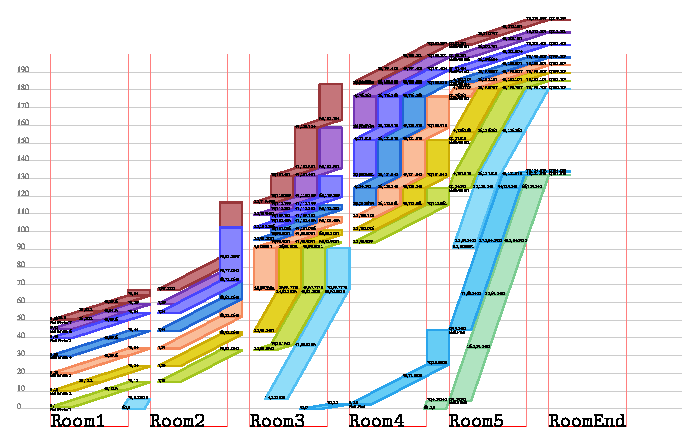
\includegraphics[angle=0,width=16cm]{50_figs/__Testing_Pipe_Zboxen.eps}
  \caption{``Balls'' moving through five ``rooms'': The time axis is
    vertical, labeled in seconds on the left, progressing upwards.
    Each ball's trajectory is a different colour. Their behaviour and
    starting points are variously described in the zsyntax input
    file. Black numbers along the trajectories are $(x,t)$ values.}
  \label{fig:balls}
\end{figure}

A Gawk program (which is unsophisticated, having some things like
labels hard-coded) is provided which extracts the movement of the
\zobj{zboxen} and plots the output in a Postscript file:\\
\comline{cat \_Testing\_Pipe\_Zboxen.zo | gawk -f Report\_to\_ps.awk > \_Testing\_Pipe\_Zboxen.eps }\\
The resulting plot is shown in \Figref{fig:balls}.

A script is provided which contains the
above commands and an additional line to convert to a PDF file.
It requires Ghostscript to be installed, as it uses {\tt ps2pdf}.
To run the example and produce also the output graph:\\
\comline{./01\_RunAndGraphResults.sh}

Mapping of report lines to segments of the plot is straightforward; for example
the first line beginning {\tt R: zbox ztype=Ball,2,1} in the {\tt .zo} file shown
corresponds to the first blue (
\includegraphics[angle=90,width=0.4cm]{50_figs/_Blue.eps})
trajectory segment visible inside {\tt Room3}. \zobj{Zbox} speeds and speed limits
are also readily visible.

In this simple example, progress of the entire simulation can be seen in a single plot.
In particular, it is to be noticed that within a \emph{Pipe}-type \zobj{zbox},
passing is not allowed, whereas in {\tt Room2} which is a \emph{Span}-type
\zobj{zbox}, overlapping trajectories are apparent.
All ball \zobj{zboxen} eventually make their way to the \emph{Sink} \zobj{zbox} {\tt RoomEnd} and quit the system.

\begin{figure}[ht]
  \centering
  \includegraphics[angle=0,width=16cm]{50_figs/__Testing_Pipe_Zboxen2.eps}
  \caption{``Balls'' moving through five rooms: The impediment {\tt Ball.Stuck} has been removed from the system.}
  \label{fig:balls2}
\end{figure}
Commenting of the line describing {\tt Ball.Stuck}
\begin{lstlisting}[mathescape]
  # [zbox Ball.Stuck A=Ball n=1  z=<Room4>  P=<RoomTour1> i_P=3 x=67.5 v=0.55]        
\end{lstlisting}
and re-running the model, the new plot shown in \Figref{fig:balls2} is obtained.
It can be seen that without the impediment that {\tt Ball.Stuck} (
\includegraphics[angle=90,width=0.4cm]{50_figs/BallStuckColour.eps})
represented, the system of rooms behaves differently.


\chapter{Metro systems}
\label{Chap:Metro}
\section{Modelling a metro system}
\label{metsys}

Reference will be made below to the various objects in the Zimulator
framework; the reader is referred to \Chapref{Chap:Zim} for
the meaning of these terms (e.g. \zobj{zbox}, \zobj{zpath}, \zobj{zlink}).

The terminology adopted here is `Metro System' and as mentioned above
this term is inexact. It is important to realize that not all metro
systems are identical, and source data for such systems may be
expressed in various ways. Therefore there is no single `correct' way
to construct a model of such a system, and the level of detail and precision
employed will vary depending on the model application and availability
of data.  In the present section will be discussed a reasonable way to
map a generic metro system to the ingredients available in the
Zimulator framework.

The system is deemed to have at least trains, stations, tracks and
passengers.  Beyond this minimum, there can be significant variation.

It is noted that while buses and the associated issues of more
extensive traffic modelling are complex and beyond the scope of this
discussion, buses travelling on dedicated or at least uncongested
traffic lanes might reasonably be interpreted as `trains' on
`tracks'. Buses in some cities are operated very much like trams or
streetcars.

Stations in some systems, like tram or LRT systems, are merely
platforms or sidewalks on which passengers may stand.  Some systems
have raised tracks and a station is thus comprised of a concourse with
platforms accessible via escalators or stairwells.  In subway systems,
a typical station is comprised of an underground concourse with
platforms at various extremedies, which concourse is accessible via a
set of tunnels leading from entrances, which might be independent, or
might connect to other structures like shopping malls or office
centres.  In some systems there are fare gates, through which
passengers walk on entry to the system; often passengers must also
pass through these when exiting. Sometimes these fare gates are part
of the station infrastructure; sometimes they are part of the vehicles
themselves.

In order that a comprehensive example be constructed below in \secref{Madrid},
here it is anticipated that a full station model will be employed.

At a high level, modelling of vehicle depots could be accomplished
within the present framework; nevertheless such modelling is
system-dependent and is not typically important from a passenger point
of view. Rather than maintain a conserved vehicle inventory via such
depot modelling, it will be seen to be sufficient to generate trains
at certain source points, and to discard these trains in sinks when
they have traversed their routes.

\subsection{Representation}
\label{sec:repr}

Objects in the system which are represented by \zobj{zboxen} are
trains, tracks, bounds, platforms, corridors, concourses, gates, `outgates'
and stations; each of these is a particular \zobj{ztype} as described in \secref{modparams} below.

A generic template for the construction of stations is shown in \Figref{fig:STN}.
\begin{figure}[ht]
  \centering
  \includegraphics[angle=0,width=12cm]{60_figs/_SeveralStations2.eps}
  \caption{
    Five stations along sections of two transit lines:
    The red \zobj{zboxen} may contain passengers; the black may contain trains.
    \zobj{zlinks} which are red allow passengers; those which are black allow trains.
    The mnemonics {\tt Stn}, {\tt Pf}, {\tt Bn}, {\tt Co}, {\tt Cc}, {\tt Gt}, {\tt Go} and {\tt Trk} refer to a \zobj{zbox}
    representing a Station, Platform, Bound, Corridor, Concourse, Gate, `GateOut' and Track Segment, respectively.
    The blue \zobj{zlink} is an implied \zobj{zlink}, between the Train {\tt T} and Bound, and is traversable by passengers.
    The circular dots represent details not shown.
    \label{fig:STN}
  }
\end{figure}

Each train, represented by a \zobj{zbox}, is deployed on a \zobj{zpath} and
successively visits \zobj{zboxen} representing track intervals and representing bounds,
which are the stops next to platforms where passengers may board or alight.

Each passenger is also a \zobj{zbox}; a passenger is created via a
\zobj{zdemand} by copying a prototype passenger and placing the
\zobj{zbox} in a gate at the station of origin. A \zobj{zpath} is
assigned which controls the subsequent travel. The
passenger\footnote{As described in detail in the Zimulator
  documentation, visiting a \zobj{zbox} implies \emph{progression}
  through it, and moving to the next \zobj{zbox} involves
  \emph{shifting} to it via a \zobj{zlink}.}  successively visits
\zobj{zboxen} representing a gate, corridor, concourse, corridor and
platform, by traversing each and then shifting via \zobj{zlink} to the
next. The passenger then shifts to a train within the bound
\zobj{zbox} associated with the platform; this is made possible
by an implicit \zobj{zlink} from the train to the bound, traversible by passengers.
If later in the trip a transfer is to be undertaken, the passenger
shifts out to a platform, then to a corridor, concourse, corridor and
new platform at the transfer station, before shifting to a train in
the bound associated with the new platform. The passenger disembarks
by shifting out of the train to a platform, then eventually to a gate
and finally an `outgate' which is a sink via which the passenger quits
the system.

In this way, a passenger's full trip from station `O' to station `D' in the diagram
would involve visiting all the shaded \zobj{zboxen}.

The station construction displayed in \Figref{fig:STN} is general enough to
model many real-world stations.  Of course, some systems are
constructed such that common transfers may be made by simply walking
across a platform; this could be modeled, for example, by instead using
a simpler structure with a short corridor \zobj{zbox} between the platforms.

It is emphasized that correct interpretation of configurations like that shown in \Figref{fig:STN}
involves recognizing that time spent by a \zobj{zbox} occurs in \emph{progressing}
through various container \zobj{zboxen}, and not in instantaneous \emph{shifting}
from one to the next along \zobj{zlinks}.

\subsection{zsyntax files}
\label{seczsyn}

The data mentioned in the previous section are used to build the metro system using \zobj{zboxen}.
The metro system is thereby specified in the zsyntax files listed below.

Separation of zsyntax simulator input into particular files is entirely arbitrary;
the simulator is simply provided with zsyntax input, and it can be stored in one or
many files as seen fit by the user. 

\subsection{Simulator input files}

The simulator expects the system to be expressed in \zobj{zsyntax}.

There are several sets of information which must be expressed in order
to model the system; these include:
\begin{itemize}
\item The \zobj{zsystem} itself (a few global parameters)
\item A number of \zobj{ztypes} covering each kind of obejcts in the system to be modeled by a \zobj{zbox}
\item Static \zobj{zboxen} describing each metro station as in \Figref{fig:STN}
\item Static \zobj{zboxen} describing each track segment in the network.
\item Static \zobj{zlinks} describing connections of the track segments to the bounds at the stations.
\item Prototype \zobj{zboxen} from which trains and passengers are created.
\item \zobj{zpaths} which describe the paths through the system taken by each train line.
\item A number of \zobj{zschedules} which indicate the times for deployment of trains on paths.
\item A number of \zobj{zdemand} objects which describe passengers with intended destinations to be injected into the system.
\end{itemize}

In \Secref{modparams} below is described the mapping between metro-system parameters and the
individual attributes of Simulator objects like \zobj{zboxen}.

In the Madrid example in \Chapref{Chap:Metro}, the above list will be distributed among
six files which will be discussed in detail.

\subsection{System parameters}
\label{modparams}
The main concept in modelling a system is that progress of a
\zobj{zbox} through its container corresponds to progression of some
modeled degree of freedom. In the case of a Track \zobj{zbox}, the
position of the Train \zobj{zbox} inside is the spatial position of
the train on that section of track; in the case of a Bound
\zobj{zbox}, the progression simply corresponds to the time taken
while the train is waiting at a Bound (i.e.~dwelling time).

In this way most of the parameters associated with the metro system are expressed
as attributes of certain \zobj{ztypes}, and so are exhibited by the
various \zobj{zboxen} in the system.

Some of these parameters are shown and described below, by extracting
example pieces of zsyntax. Since these extracts are not in context,
the particular numerical values (e.g. {\tt L=1380} or {\tt S=100}) are
unimportant and are merely illustrative.

Model parameters represented in the {\tt Train} \zobj{ztype} include train capacity and train speed:
\begin{lstlisting}[mathescape]
  [ztype A=Train n=1 q=1 C={Pax 1} m=Bag l=30 L=1380 N=1380 S=0 $\chi$=<TrainDoors>
    v=20 R=S]
\end{lstlisting}
\begin{itemize}
\item {\tt m=Bag} -- Passengers need not traverse when contained in a train.
\item {\tt L=1380} or {\tt N=1380} -- controls the capacity of a
  train. If $L$ is used, then it is measured in the same units as {\tt Pax}.$l$.
  Train capacity could be determined via some kind of calibration, and will be discussed later.
\item {\tt v=20} -- Speed of a train. Length units match those of {\tt Track}.$L$, and $m/s$ are used here.
\item {\tt S=0} -- Space `between' passengers.
\end{itemize}

Model parameters represented in the {\tt Bound} \zobj{ztype} include dwelling time:
\begin{lstlisting}[mathescape]
  [ztype A=Bound n=1  m=Pipe C={Train 1} L=45 V=1 N=1]
\end{lstlisting}
\begin{itemize}
\item {\tt m=Pipe} -- Controls how trains may stop at a bound.
\item {\tt L=45} -- Controls how long a train stops at a bound, in conjunction with {\tt Train}.$v$ and {\tt Train}.$l$.
\item {\tt V=1} -- Limiting velocity for trains; this limits {\tt Train}.$v$.
\end{itemize}
The dwelling time in this example is 30 s; since the train has length 30, it can progress 15 out of 45 with limited velocity 1.

Model parameters represented in {\tt Track} include travel time between stations:
\begin{lstlisting}[mathescape]
  [ztype A=Track n=1 m=Pipe C={Train 1} L=1000 S=100]
\end{lstlisting}
\begin{itemize}
\item {\tt m=Pipe} -- Trains may not pass each other on a track.
\item {\tt L=1000} -- The distance between two subsequent stations. This is overridden in specific \zobj{zboxen} of this \zobj{ztype}.
\item {\tt S=100} -- Minimal distance between successive trains.
\end{itemize}

Model parameters represented in {\tt Concourse} and {\tt Corridor} include walking distances within stations:
\begin{lstlisting}[mathescape]
  [ztype A=Concourse n=1 m=Bag C={Pax 1} N=10000]
  [ztype A=Corridor n=1 m=Span C={Pax 1} L=200 W=10]
\end{lstlisting}  
\begin{itemize}
\item {\tt L=200 W=10} -- Capacity of a corridor will be 2000 passengers. The walking distance through is 200 m.
  These are overridden by each {\tt Co} \zobj{zbox}. In particular, $L$ could be determined via calibration.
\item {\tt N=10000} -- The capacity of the {\tt Concourse} is typically overestimated in order not to
  produce an artificial bottleneck in the system.
\end{itemize}
The walking \emph{times} within the system are then determined by passenger walking speeds, which
are specified either as an attribute of a prototype Passenger within a \zobj{zsource} inside
\zobj{zdemand}, or specified within the \zobj{zsource} as the parameters of a log-normal
distribution.

Model parameters represented in {\tt Platform}:
\begin{lstlisting}[mathescape]
  [ztype A=Platform n=1 m=Bag C={Pax 1} L=4000]
\end{lstlisting}
\begin{itemize}
\item {\tt m=Bag} -- Passengers do not traverse a platform; they simply wait there.
\item {\tt L=4000} -- Capacity of a platform. This is not usually important for simulation, unless there is special interest in saturation of platforms.
\end{itemize}

The \zobj{ztypes} of {\tt Gate} and {\tt Platform} have a containment type of `Bag', thereby having only capacity
but no traversal attributes.

%\subsection{Simulation output}
%...

\subsection{Calibration}

In very general terms, there may be `ground truth' sources of data
which can be used to calibrate aspects of the simulation. For example,
there may be sensors on train platforms which can be used to calibrate
[effective] train speeds. There may be a farecard system which records
the precise times of passengers `tapping' in an out of the system;
this could be used to calibrate not only train speeds but also walking
times within the system and possibly other properties like effective
train capacities.

In section \secref{Chap:MadCali} an illustrative example of such
calibration will be given, calibrating the two-parameters of the
log-normal distribution used for passenger walking speeds.  Although
the system approximately modeled is a real-world system, the
`ground-truth' data utilised will be synthetic.


\chapter{Madrid Metro}
\label{Chap:Madrid}
\section{Madrid Metro}
\label{Madrid}

In this chapter will be developed a Zimulator model for the Madrid
Metro system.  The model is to be constructed using only public
sources of data, which are in cases of insufficiency supplemented with
synthetic data.  The resultant model is intended here solely to
function as an illustrative example of metro-system simulation.

All public data are extracted from Wikipedia.\footnote{Data are taken from \href{https://en.wikipedia.org/wiki/Madrid_Metro}{https://en.wikipedia.org/wiki/Madrid\_Metro} and associated pages.} All source addresses are included
as fields within the raw metro-system data files described below.

The level of detail of the model will be influenced by the form and
details of available data. Such a model is sufficient for illustrative
purposes; in the case of quantitative application to a metro system,
actual system data would be expected to produce a more realistic model.

\subsection{Metro system public data}

Available data describe the geometrical layout of the metro network,
in addition to the transit lines and connectivity. The extracted data
have been stored in three source files, the form of which is briefly
described here. This file format is nothing more than an intermediate
tool to create the zsyntax files which describe the system. It is a
simple ad-hoc format particular to the Madrid system, but may be
useful, with possible embellishments, in describing other metro
systems.

{\tt Line\_List.csv} -- This defines an index, code, name and source location for each of the 16 metro lines. 
An example row is: 
\begin{lstlisting}[mathescape]
  11,s,L11,Plaza Elíptica - La Fortuna,https://en.wikipedia.org/wiki/Line_11_(Madrid_Metro)
\end{lstlisting}
The field `s' indicates that the line is `straight' as opposed to a loop line, which would be indicated by `l'.

{\tt Station\_List.csv} -- This defines a three-letter code, name, latitude and longitude for each metro station. \\
An example row is:
\begin{lstlisting}[mathescape]
 SLS,San Lorenzo,40.4744713,-3.6395754,https://en.wikipedia.org/wiki/San_Lorenzo_(Madrid_Metro)
\end{lstlisting}  
The three-letter codes are generated for the purpose of the simulation, and are not official.

{\tt Itinerary\_List.csv} -- This file defines the paths taken by each line in the system, as a list of stations.
An example sequence of rows is:
\begin{lstlisting}[mathescape]
 5,1,ADO,0
 5,2,ECE,802.249
 5,3,LEA,1407.06
 . . .
 5,30,PAL,735.651
 5,31,CAT,579.064
 5,32,CDC,1226.36
\end{lstlisting}
This section of 32 rows in total indicates that transit line number 5 travels through
32 stops, from ADO to CDC.  The fourth field indicates the distance
in metres to the given stop from the previous stop.  In the present
case the distances have been estimated using the latitude and
longitude coordinates of each station, taking the geodesic distance
and multiplying arbitrarily by $1.1$.

These CSV files will be taken to be the raw system data; below in \secref{madseczsyn}
these data will be used to engineer the system in terms of Zimulator objects.

\subsection{Synthetic data}

The data mentioned in the previous section do not describe the system
comprehensively; while the infrastructure is thereby specified, the
supply and demand remain undetermined. These are generated synthetically.

\begin{figure}[ht]
  \centering
  \includegraphics[angle=0,width=8cm]{70_figs/_headway_vs_ToD.eps}
  \caption{Headway depends on time of day.}
  \label{hwdep}
\end{figure}

\begin{figure}[ht]
  \centering
  \includegraphics[angle=0,width=10cm]{70_figs/_SystemFlows.eps}
    \caption{Large-scale demand throughout the day.
      The figure shows the directional local net flow of passengers in a two-dimensional plane,
      at various times during the day. For spatial reference, a schematic of the
      transit lines is shown below the first slice. }        
  \label{demandinday}
\end{figure}
  
Trains are supplied on each of the lines at intervals, all day long
from approximately 04:30 to 25:00. The headway, shown in
\Figref{hwdep}, (time between subsequent train deployments) is modeled
very simply, to accommodate a higher train frequency during peak hours
of near 07:00 and 19:00.

The passenger demand is generated to represent the general flow within
an urban area; the flow of commuters is generally towards the city
centre during the morning peak period, and generally away from the
centre during the evening peak. There is no intention to model accurately the
flow in the actual city; the intention here is to provide an example day of
demand which is not entirely unrealistic. The sequence of passenger
flows throughout the day is indicated in \Figref{demandinday}.

\subsection{Station template}

The arrangement of each station in the metro system is that presented
earlier in \Figref{fig:STN}, with four gates associated with each
station. This is an arbitrary choice. At a station at which $n$ transit
lines stop, there are $2n$ platforms, so as to accommodate each
direction of each line.  In a more detailed model, the number of
gates, number of platforms, and also the connectivity among them could
be adjusted to reflect actual station layout.

\subsection{zsyntax files}
\label{madseczsyn}

The data mentioned in the previous section are used to build the metro system using \zobj{zboxen}.
The Metro system is thereby specified in the zsyntax files listed below.

Separation of zsyntax input into particular files is entirely arbitrary;
the simulator is simply provided with zsyntax input, and it can be stored in one or
many files as seen fit by the user. 

\begin{itemize}
\item {\tt 00\_StaticTypes.zim} -- defines overall system and \zobj{ztypes} for all objects.
\item {\tt \_01\_Stations.zim} -- contains a description of all stations.
\item {\tt \_02\_Tracks.zim} --  defines all tracks and their connections to stations. 
\item {\tt \_03\_Paths.zim} --  defines the paths through the system which are followed by trains.
\item {\tt \_04\_Schedules.zim} --  specifies the times at which trains are deployed.
\item {\tt \_05\_Demand.zim} -- contains \zobj{zdemand} objects describing deployment of passengers during the day.
\end{itemize}

In the following subsections the content of each of these zsyntax input files will be explained in detail.

\subsubsection{Static types: {\tt 00\_StaticTypes.zim}}

The \zobj{zsystem} is defined, with particular reference and simulation times, and a certain level of reporting:
\begin{lstlisting}[mathescape]
[zsystem Madrid T_0=0 t_0=05:00 t_1=23:00 $\Delta$t=600.0 R=S ]
\end{lstlisting}
The \zobj{ztypes} in the system are next defined. A discussion of how
the values specified here relate to metro-system parameters such as
dwelling times and walking speeds can be found above in
\secref{modparams}.

There are \zobj{ztypes} for dynamical objects in the system:
\begin{lstlisting}[mathescape] 
  [ztype A=Pax n=1 v=2.0 l=1 R=S2
    Z={ Train 1 Platform 1 Concourse 1 Corridor 1 } ]
  [ztype A=Train n=1 q=1 C = { Pax 1 } m=Bag l=100 L=1380
    N=1380 S=0 $\chi$=<TrainDoors> v=21.04 R=S1d ]
\end{lstlisting}
Passengers may \emph{sleep}, as described in \Chapref{Chap:Zim}, when waiting inside certain containers.
The train capacity and size could be over-ridden by trains deployed on each line.

A number of objects are able to contain passengers:
\begin{lstlisting}[mathescape] 
  [ztype A=Station n=1 C={ Concourse 1 Gate 1
      OutGate 1 Platform 1 Bound 1 Corridor 1 } ]
  [ztype A=Platform n=1 m=Bag C={Pax 1} N=3000 ]
  [ztype A=Concourse n=1 m=Bag C={Pax 1} N=3000 ]
  [ztype A=Corridor n=1 m=Span C={Pax 1} L=200 W=5 ]
  [ztype A=Gate n=1 m=Bag C={Pax 1} $\$$=2 ]
  [ztype A=OutGate n=1 C={ Pax 1 } m=Sink ]
\end{lstlisting}
These lines define that a {\tt Station} may contain a number of other objects, and then define those object types,
in correspondence with the station model which was chosen earlier.
The capacity for the Platform, Concouse and Corridor could be overridden at each station if more detail were required.

Passengers will utilise the above objects; trains will utilise the following.
\begin{lstlisting}[mathescape] 
  [ztype A=Bound n=1 m=Pipe C={Train 1} L=124 V=1 N=1 ]
  [ztype A=Track n=1 m=Pipe C={Train 1} L=1000 S=100 ]
\end{lstlisting}
The $L$ parameter for a Bound determines the dwelling time at the platform.
The length of $1000$ for a Track is always over-ridden with an actual track length,
as shown below.

Finally, the types for train sources and sinks are defined:
\begin{lstlisting}[mathescape] 
  [ztype A=TrainSink n=1 C={ Train 1 } m=Sink ]
  [ztype A=TrainSource n=1 m=Bag C={Train 1} ]
  [zlink TrainDoors A={ Pax 1 0 } ]
\end{lstlisting}
The last row here describes the implicit \zobj{zlink} which connects a train to its container.
As described earlier, this is utilised by passengers when the train is inside a bound \zobj{zbox}
for boarding or alighting.

\subsubsection{Station descriptions: {\tt \_01\_Stations.zim}}

This file contains a specification of every station in the metro system.
As an example of a single such station:
\begin{lstlisting}[mathescape] 
# ----------- Station: PDA -- Puerta de Arganda -----------
[zbox PDA i=latlon:40.4013157,-3.5959768 A=Station n=1 ]
[zbox PDA_Cc A=Concourse n=1 z=<PDA> ]
# ----------- Gates for PDA
[zlink $\mu$=<PDA_Cc> $\nu$=<PDA_GtCo_1> A={ Pax . 0 } ]
[zbox PDA_GtCo_1 A=Corridor n=1 L=110 z=<PDA> ]
[zlink $\mu$=<PDA_GtCo_1> $\nu$=<PDA_Gt_1> A={ Pax . 0 } ]
[zbox PDA_Gt_1 A=Gate n=1 z=<PDA> ]
[zlink $\mu$=<PDA_Gt_1> $\nu$=<PDA_Gt_1_out> A={ Pax . 0 } ]
[zbox PDA_Gt_1_out A=OutGate n=1 z=<PDA> ]
[zlink $\mu$=<PDA_Cc> $\nu$=<PDA_GtCo_2> A={ Pax . 0 } ]
[zbox PDA_GtCo_2 A=Corridor n=1 L=120 z=<PDA> ]
[zlink $\mu$=<PDA_GtCo_2> $\nu$=<PDA_Gt_2> A={ Pax . 0 } ]
[zbox PDA_Gt_2 A=Gate n=1 z=<PDA> ]
[zlink $\mu$=<PDA_Gt_2> $\nu$=<PDA_Gt_2_out> A={ Pax . 0 } ]
[zbox PDA_Gt_2_out A=OutGate n=1 z=<PDA> ]
[zlink $\mu$=<PDA_Cc> $\nu$=<PDA_GtCo_3> A={ Pax . 0 } ]
[zbox PDA_GtCo_3 A=Corridor n=1 L=130 z=<PDA> ]
[zlink $\mu$=<PDA_GtCo_3> $\nu$=<PDA_Gt_3> A={ Pax . 0 } ]
[zbox PDA_Gt_3 A=Gate n=1 z=<PDA> ]
[zlink $\mu$=<PDA_Gt_3> $\nu$=<PDA_Gt_3_out> A={ Pax . 0 } ]
[zbox PDA_Gt_3_out A=OutGate n=1 z=<PDA> ]
[zlink $\mu$=<PDA_Cc> $\nu$=<PDA_GtCo_4> A={ Pax . 0 } ]
[zbox PDA_GtCo_4 A=Corridor n=1 L=140 z=<PDA> ]
[zlink $\mu$=<PDA_GtCo_4> $\nu$=<PDA_Gt_4> A={ Pax . 0 } ]
[zbox PDA_Gt_4 A=Gate n=1 z=<PDA> ]
[zlink $\mu$=<PDA_Gt_4> $\nu$=<PDA_Gt_4_out> A={ Pax . 0 } ]
[zbox PDA_Gt_4_out A=OutGate n=1 z=<PDA> ]
\end{lstlisting}
The {\tt i} field encodes information which will simply pass through the
Zimulator unprocessed; the station latitude and longitude is useful
for simple plotting of output data.
The remainder of the station is a set of static \zobj{zboxen} and \zobj{zlinks}
as described in \secref{sec:repr} and shown in \Figref{fig:STN}.

\subsubsection{Track network: {\tt \_02\_Tracks.zim}}

This file contains a description of all tracks which link stations,
along each metro line's route. It is noted that lines (apparently) do not
share track segments within the Madrid system; if this were the case
then generation of this file would be slightly more complex.
The first few lines of the file follow:
\begin{lstlisting}[mathescape]
# ----------- Line L1(Pinar de Chamartín - Valdecarros) :
[zbox Train_proto/L1 A=Train n=1 $\pi$=1 z=<Source_L1>]
[zsource Train_Source_L1 $\phi$=<Train_proto/L1> m=One o=Container ]
[zbox Source_L1 A=TrainSource n=1 ]
[zbox Sink_L1 A=TrainSink n=1 ]
\end{lstlisting}
Each metro line has its own prototype Train \zobj{zbox} and Train \zobj{zsource}, which are used to
deploy `fresh' trains on the line. The prototype train is contained in the \zobj{zbox} labeled {\tt Source\_L1},
and then copied to produce deployed trains which begin in this same container.
Each metro line also has its own sink, where trains which have run the whole line quit the system.
The next few lines of the file are:
\begin{lstlisting}[mathescape]
[zbox Trk_L1_0_PDC_BBA L=978.921 A=Track n=1
  i=latlon2:40.4801375,-3.6667999,40.4768117,-3.6763701 ]
[zlink $\mu$=<PDC_Bn_L1_0> $\nu$=<Trk_L1_0_PDC_BBA> A={ Train . 1 } ]
[zlink $\mu$=<Trk_L1_0_PDC_BBA> $\nu$=<BBA_Bn_L1_0> A={ Train . 1 } ]
[zbox Trk_L1_0_BBA_CCH L=822.981 A=Track n=1
  i=latlon2:40.4768117,-3.6763701,40.472101,-3.6826857 ]
[zlink $\mu$=<BBA_Bn_L1_0> $\nu$=<Trk_L1_0_BBA_CCH> A={ Train . 1 } ]
[zlink $\mu$=<Trk_L1_0_BBA_CCH> $\nu$=<CCH_Bn_L1_0> A={ Train . 1 } ]
[zbox Trk_L1_0_CCH_AIA L=878.787 A=Track n=1
  i=latlon2:40.472101,-3.6826857,40.4668983,-3.6891989 ]
[zlink $\mu$=<CCH_Bn_L1_0> $\nu$=<Trk_L1_0_CCH_AIA> A={ Train . 1 } ]
[zlink $\mu$=<Trk_L1_0_CCH_AIA> $\nu$=<AIA_Bn_L1_0> A={ Train . 1 } ]
\end{lstlisting}
These represent the track segments travelling from PDC to BBA,  BBA to CCH and CCH to AIA stations.
Each of these segments is connected via \zobj{zlinks} to the Bound \zobj{zbox} at the station at each end.
This is an implementation of the diagram in \Figref{fig:STN}, with trains expected to subsequently
visit Bound and Track \zobj{zboxen}.
As with Station \zobj{zboxen}, the {\tt i} field is unused by the simulator, but appears in output as
a convenience.

\subsubsection{Train trajectories: {\tt \_03\_Paths.zim}}

Train \zobj{zboxen} follow \zobj{zpaths} through the system which are defined here.
An example \zobj{zpath} from this file is:
\begin{lstlisting}[mathescape]
# ----------- Line ML1_1(Pinar de Chamartín - Las Tablas) complete path:
[zpath Train_ML1_1_Line A=Train n=1 m=Open $\Lambda$={ [zs $\phi$=<LTL_Bn_ML1_1>]
 [zs $\phi$=<Trk_ML1_1_LTL_LAE>] [zs $\phi$=<LAE_Bn_ML1_1>] [zs $\phi$=<Trk_ML1_1_LAE_MTM>]
 [zs $\phi$=<MTM_Bn_ML1_1>] [zs $\phi$=<Trk_ML1_1_MTM_BIB>] [zs $\phi$=<BIB_Bn_ML1_1>]
 [zs $\phi$=<Trk_ML1_1_BIB_LDV>] [zs $\phi$=<LDV_Bn_ML1_1>] [zs $\phi$=<Trk_ML1_1_LDV_IOS>]
 [zs $\phi$=<IOS_Bn_ML1_1>] [zs $\phi$=<Trk_ML1_1_IOS_VDC>] [zs $\phi$=<VDC_Bn_ML1_1>]
 [zs $\phi$=<Trk_ML1_1_VDC_FDL>] [zs $\phi$=<FDL_Bn_ML1_1>] [zs $\phi$=<Trk_ML1_1_FDL_PDC>]
 [zs $\phi$=<PDC_Bn_ML1_1>]  [zs $\phi$=<Sink_ML1>] } ]
\end{lstlisting}
This defines the trajectory for the ML1 line, travelling in direction
1. (Arbitrarily the two directions along a route have been termed 0
and 1.) Within ths \zobj{zpath} are 18 \zobj{zstop} objects,
referencing \zobj{zboxen} corresponding to alternating Bounds and Tracks in
succession. Lastly, the Sink for the ML1 line is visited. A train
following such a \zobj{zpath} will quit the system upon arrival there.

\subsubsection{Train schedules: {\tt \_04\_Schedules.zim}}

Here are expressed all the times during the day when a train is to be deployed
on each of the metro lines. This is done with a \zobj{zschedule} object
for each line, for example:
\begin{lstlisting}[mathescape]
[zschedule Sch_ML3_1 T_0 = 0 T={ 15618 15897 16169 16434 16692 16943 17188
 . . . . . 
 89065 89524 89990 } S=<Train_Source_ML3> P=<Train_ML3_1_Line> ]
\end{lstlisting}
The provided source is the \zobj{zsource} defined for the metro line, ML3 in this case.
The path given the Train will be the ML3 direction-1 \zobj{zpath}.
It can be seen that the first train to be deployed on ML3 will be at 4:20:18.

\subsubsection{Passenger demand: {\tt \_05\_Demand.zim}}

In this example, the passengers are all provided at once in a single \zobj{zdemand} object which looks like the following:
\begin{lstlisting}[mathescape]
[zdemand Madrid_Day_pax
  S=[zsource Pax_Src $\phi$=[zb Pax A=Pax n=1 $\pi$=1] m=One o=Teleport]
  T_0=0 Reference=%s
  L={ <TDM_Gt_1> <TDM_Gt_1_out> <TDM_Gt_2> <TDM_Gt_2_out>
    <TDM_Gt_3> <TDM_Gt_3_out> <TDM_Gt_4> <TDM_Gt_4_out>
    <RAR_Gt_1> <RAR_Gt_1_out> <RAR_Gt_2> <RAR_Gt_2_out> <RAR_Gt_3> <RAR_Gt_3_out>
    . . . 
    <DEL_Gt_1> <DEL_Gt_1_out> <DEL_Gt_2> <DEL_Gt_2_out>
    <DEL_Gt_3> <DEL_Gt_3_out> <DEL_Gt_4> <DEL_Gt_4_out>
  }
  D={ 
    1972 1671 14400 1
    . . .
    294 1563 89999 1
  } # total of 1750015 passengers for the day.
]
\end{lstlisting}
A \zobj{zsource} from which to procure `fresh' passengers is provided,
within which is a prototype passenger \zobj{zbox}.  Of course, these
could have been provided elsewhere (say, in {\tt 00\_StaticTypes.zim})
and referenced, but as they are conceptually express attributes of the
demand, they appear here in-line.

{\tt L} is a list of \zobj{zboxen} in the system which can be specified as origins or destinations
for the Passengers deployed. Conveniently, even indices correspond to origins, while odd indices
correspond to destinations; this is merely a convention.

{\tt D} specifies a list of passengers to deploy; each set of four numbers
specifies an origin and destination index in the set $L$, a time of
day, and a number of passengers.

\subsection{Running the simulation}

The model can be run using the command-line interface to the core
simulator.  The resulting reporting output will be parsed and analysed
in \Secref{sec:metzimout} below. In the present section, it will be
shown how to produce and interpret verbose output during a simulation;
this is useful in `debugging' while assembling a model of a metro
system and understanding that it functions as intended.

A bash script {\tt 02\_Run\_simulation.sh} is provided, which simply contains (without {\tt z=30}) the command
\begin{lstlisting}[mathescape]
java  -jar CL.jar -razo z=30 zl=45 I=00_StaticTypes.zim \
             I=_01_Stations.zim    I=_02_Tracks.zim \
             I=_03_Paths.zim       I=_04_Schedules.zim \
             I=_05_Demand.zim      R=out/madrid_01.zo
\end{lstlisting}
indicating that the above collection of input files is to be used to generate an output { \tt madrid\_01.zo}.
While the simulation is running, the system status will be displayed on the terminal every 30 seconds,
up to a maximum of 45 rows of text.
The simulation could equivalently be run via: \\
\comline{./02\_Run\_Simulation.sh z=30}

Since periodic verbose updates have been enabled with {\tt z=30}, as
the simulation runs the terminal will display output like the following.

%\vspace{0.5cm}
%
% \input{Madrid_z30.tex}   % We choose the picture approach instead.
%
\includegraphics[angle=270,width=13cm]{70_figs/Madrid_z30.eps}
\vspace{0.5cm}

Some of the information pertains only to internal degrees of freedom,
but generally the output is intended to indicate progress of the simulation,
especially during debugging of a system.

$X=2130$ indicates that 2130 passes of the system have been computed.
The base time $T_0$ and simulation window $(t_0,t_1)$ are indicated,
as is the current simulation time $t$. In this example, at $t=$05:11:30
the simulation is 1.06\% complete, running at a relative speed of $133.48\times$
(i.e. the simulator is running this factor faster than reality),
and has averaged a relative speed of $95.34\times$ so far. The latest number
of passes $N[0]$ of the $[0]$ system list required for state
resolution is $4$. The indicator `marks' is not of interest to the user.

The columns $[0]$, $[T]$, $[Z]$ and $[S]$ are the four
`Syslists' which are maintained internally, representing \zobj{zboxen}
which are either in discrete states, timed states, sleeping, or
static, respectively. The $\in$ symbols, when present, indicate
first-level containment. In this example, there are 32236 Passenger \zobj{zboxen},
distributed among Gates, Platforms, Corridors and Trains. 1104 of them
happen to be riding trains at 05:11:30.

This $z=30$ display is one method of seeing how the system is
developing.  Another way is to enable \emph{verbosity}. As described,
verbosity (as distinguished from \emph{reporting}) is not intended to
be parsed by machine, but is another method by which a human can
monitor a running simulation.

\comline{./02\_Run\_simulation.sh -v}

The result is that many, many rows of output will be dumped to the terminal,
indicating information about \zobj{zboxen} and other objects and their
state transitions.

Passengers in the present model are generated via the prototype
passenger \zobj{zbox} {\tt $\varphi$=[zb Pax A=Pax n=1 $\pi$=1]}.
Therefore, the \zobj{zdemand} gives them labels based on this
\zobj{zbox} label; they will be {\tt Pax/1}, {\tt Pax/2}, etc.
A single such passenger can be followed by specifying that
verbosity should be applied only to one label. Following the
progress of passenger, say, 6502 in this way can be thus accomplished with:

\comline{./02\_Run\_simulation.sh v=Pax/6502}

which produces on the terminal a number of rows narrating the life and times of that
particular passenger:\\
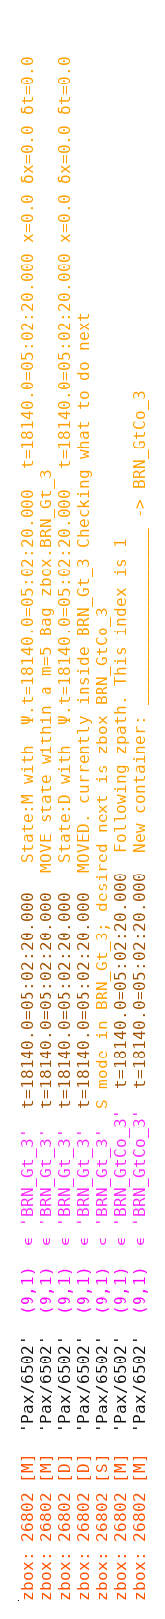
\includegraphics[angle=270,width=16cm]{70_figs/Pax_6502a.eps}\\
\vspace{0.1cm}\\
. . . (many lines)\\
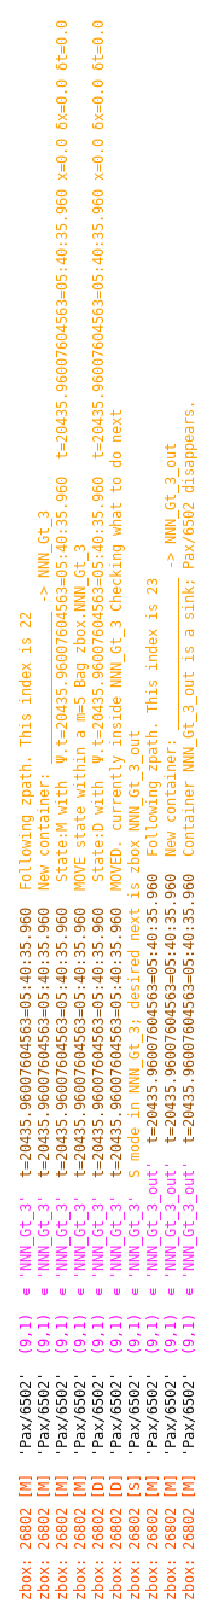
\includegraphics[angle=270,width=16cm]{70_figs/Pax_6502b.eps}\\
\vspace{0.5cm}

It is noted that the Passenger ends his trip by quitting the system at a \emph{Sink} {\tt NNN\_Gt\_3\_out} as expected.
Transitions to a new container always contain the line of several underscores; it is easier to follow the
progress of {\tt Pax/6502} by:\\
\comline{./02\_Run\_simulation.sh v=Pax/6502 | grep \_\_\_\_\_}\\
which appears on the terminal as:\\
\includegraphics[angle=270,width=16cm]{70_figs/Pax_6502.eps}
\vspace{0.5cm}

It is apparent that the passenger travelled from station BRN on {\tt Train\_proto/ML2/1} to station CJC,
then from CJC on {\tt Train\_proto/L10/7} to TTR, and finally on {\tt Train\_proto/L1/12} until
NNN where he quit the system via {\tt NNN\_Gt\_3}.

To follow the trajectory of one of these trains,\\
\comline{./02\_Run\_simulation.sh v=Train\_proto/L10/7 | grep \_\_\_\_\_}\\
which produces the terminal output:\\
\includegraphics[angle=270,width=16cm]{70_figs/Train_L10_7.eps}
\vspace{0.5cm}

The train follows the trajectory expected of a \zobj{zbox} following the
{\tt Train\_L10\_1\_Line} \zobj{zpath}, which from the zsyntax file {\tt \_03\_Paths.zim}
looks like this:
\begin{lstlisting}[mathescape]
# ---- Line L10_1(Hospital Infanta Sofía - Tres Olivos - Puerta del Sur)
[zpath Train_L10_1_Line A=Train n=1 m=Open
 $\Lambda$={ [zs $\phi$=<DEL_Bn_L10_1>]  [zs $\phi$=<Trk_L10_1_DEL_JVJ>]  [zs $\phi$=<JVJ_Bn_L10_1>]
 [zs $\phi$=<Trk_L10_1_JVJ_CVC>]  [zs $\phi$=<CVC_Bn_L10_1>]  [zs $\phi$=<Trk_L10_1_CVC_AEA>]
 [zs $\phi$=<AEA_Bn_L10_1>]  [zs $\phi$=<Trk_L10_1_AEA_CJC>]  [zs $\phi$=<CJC_Bn_L10_1>]
 [zs $\phi$=<Trk_L10_1_CJC_CDC>]  [zs $\phi$=<CDC_Bn_L10_1>]  [zs $\phi$=<Trk_L10_1_CDC_ATÁ>]
 [zs $\phi$=<ATÁ_Bn_L10_1>]  [zs $\phi$=<Trk_L10_1_ATÁ_LAG>]  [zs $\phi$=<LAG_Bn_L10_1>]
 [zs $\phi$=<Trk_L10_1_LAG_PPP>]  [zs $\phi$=<PPP_Bn_L10_1>]  [zs $\phi$=<Trk_L10_1_PPP_PDE>]
 [zs $\phi$=<PDE_Bn_L10_1>]  [zs $\phi$=<Trk_L10_1_PDE_TTR>]  [zs $\phi$=<TTR_Bn_L10_1>]
 [zs $\phi$=<Trk_L10_1_TTR_AMN>]  [zs $\phi$=<AMN_Bn_L10_1>]  [zs $\phi$=<Trk_L10_1_AMN_GMG>]
 [zs $\phi$=<GMG_Bn_L10_1>]  [zs $\phi$=<Trk_L10_1_GMG_NMN>]  [zs $\phi$=<NMN_Bn_L10_1>]
 [zs $\phi$=<Trk_L10_1_NMN_SAA>]  [zs $\phi$=<SAA_Bn_L10_1>]  [zs $\phi$=<Trk_L10_1_SAA_CCU>]
 [zs $\phi$=<CCU_Bn_L10_1>]  [zs $\phi$=<Trk_L10_1_CCU_AIA>]  [zs $\phi$=<AIA_Bn_L10_1>]
 [zs $\phi$=<Trk_L10_1_AIA_CCH>]  [zs $\phi$=<CCH_Bn_L10_1>]  [zs $\phi$=<Trk_L10_1_CCH_BBE>]
 [zs $\phi$=<BBE_Bn_L10_1>]  [zs $\phi$=<Trk_L10_1_BBE_FFU>]  [zs $\phi$=<FFU_Bn_L10_1>]
 [zs $\phi$=<Trk_L10_1_FFU_TOT>]  [zs $\phi$=<TOT_Bn_L10_1>]  [zs $\phi$=<Trk_L10_1_TOT_TEM>]
 [zs $\phi$=<TEM_Bn_L10_1>]  [zs $\phi$=<Trk_L10_1_TEM_LTL>]  [zs $\phi$=<LTL_Bn_L10_1>]
 [zs $\phi$=<Trk_L10_1_LTL_RDL>]  [zs $\phi$=<RDL_Bn_L10_1>]  [zs $\phi$=<Trk_L10_1_RDL_LAA>]
 [zs $\phi$=<LAA_Bn_L10_1>]  [zs $\phi$=<Trk_L10_1_LAA_MAE>]  [zs $\phi$=<MAE_Bn_L10_1>]
 [zs $\phi$=<Trk_L10_1_MAE_MDL>]  [zs $\phi$=<MDL_Bn_L10_1>]  [zs $\phi$=<Trk_L10_1_MDL_MDF>]
 [zs $\phi$=<MDF_Bn_L10_1>]  [zs $\phi$=<Trk_L10_1_MDF_ATL>]  [zs $\phi$=<ATL_Bn_L10_1>]
 [zs $\phi$=<Trk_L10_1_ATL_RCR>]  [zs $\phi$=<RCR_Bn_L10_1>]  [zs $\phi$=<Trk_L10_1_RCR_HIS>]
 [zs $\phi$=<HIS_Bn_L10_1>]  [zs $\phi$=<Sink_L10>]
}]
\end{lstlisting}

Two points are emphasized here. Firstly, in each of the above runs, the full simulation is indeed
being executed; the {\tt -v} option and the {\tt v=...} merely determine
levels of verbosity for either the system as a whole or individual \zobj{zboxen}.
Secondly, the above output is (as mentioned repeatedly) not intended
to be parsed beyond debugging of the system specification.
The \emph{reporting} output, which is indeed intended for this purpose,
is investigated below.

\subsection{Simulation output}
\label{sec:metzimout}

Upon completion (which is most efficiently accomplished without {\tt
  -v}), the file {\tt madrid\_01.zo} will contain the \emph{reporting}
output, every row beginning with {\tt R:}. It is of course much
like the example reporting output exhibited in \Chapref{Chap:SysExm}.

\begin{lstlisting}[mathescape]
R: zbox  i=latlon:40.4123454,-3.70466 ztype=Station,1,1 t=18000.0 R=- state=M
  Z.n=19 label=TDM t0=18000.0 x0=-0.0 t1=18000.0 x1=-0.0 $\delta$t=0.0 l=1 L=0
  Z.n=19 SpaceInside=-55 Z={ TDM_Cc(2,1) TDM_GtCo_1(8,1) TDM_Gt_1(3,1)
    TDM_Gt_1_out(4,1) TDM_GtCo_2(8,1) TDM_Gt_2(3,1) TDM_Gt_2_out(4,1)
    TDM_GtCo_3(8,1) TDM_Gt_3(3,1) TDM_Gt_3_out(4,1) TDM_GtCo_4(8,1)
    TDM_Gt_4(3,1) TDM_Gt_4_out(4,1) TDM_Bn_L1_0(6,1) TDM_Pf_L1_0(5,1)
    TDM_PfCo_L1_0(8,1) TDM_Bn_L1_1(6,1) TDM_Pf_L1_1(5,1) TDM_PfCo_L1_1(8,1)}
R: zbox ztype=Concourse,2,1 t=18000.0 R=- state=M Z.n=0 label=TDM_Cc
  z.label=TDM z.L=0 z.W=1 t0=18000.0 x0=0.0 t1=18000.0 x1=0.0 $\delta$t=0.0 l=1 L=0 z.n=19
R: zbox ztype=Corridor,8,1 t=18000.0 R=- state=M Z.n=0 label=TDM_GtCo_1
  z.label=TDM z.L=0 z.W=1 t0=18000.0 x0=0.0 t1=18000.0 x1=0.0 $\delta$t=0.0 l=1 L=110 z.n=19
R: zbox ztype=Gate,3,1 t=18000.0 R=- state=M Z.n=0 label=TDM_Gt_1 z.label=TDM z.L=0
  z.W=1 t0=18000.0 x0=0.0 t1=18000.0 x1=0.0 $\delta$t=0.0 l=1 L=0 z.n=19

  . . . (many rows)

R: zbox ztype=Train,9,1 t=38338.9315589354 R=- state=M Z.n=32 label=Train_proto/L6/15
  z.label=MLM_Bn_L6_0 z.L=124 z.W=1 t0=38338.9315589354 x0=0.0 t1=38338.9315589354
  x1=0.0 $\delta$t=0.0 l=100 L=1380 Z.n=32 SpaceInside=1348 D="⤷ MLM_Bn_L6_0"
R: zbox ztype=Train,9,1 t=38338.9315589354 R=- state=M Z.n=0 label=Train_proto/L6/57
  z.label=Trk_L6_0_MLM_PPA z.L=749 z.W=1 t0=38338.9315589354 x0=0.0 t1=38341.260456273805
  x1=49.0 $\delta$t=2.328897338403042 l=100 L=1380 Z.n=0 SpaceInside=1380 D=""
R: zbox ztype=Train,9,1 t=38338.9315589354 R=- state=D Z.n=32 label=Train_proto/L6/15
  z.label=MLM_Bn_L6_0 z.L=124 z.W=1 t0=38338.9315589354 x0=0.0 t1=38362.9315589354
  x1=24.0 $\delta$t=24.0 l=100 L=1380 Z.n=32 SpaceInside=1348 D=""  
\end{lstlisting}
with these reporting rows indicating each \zobj{zbox} movement which occured during the
simulation. Since the command-line interface has been used, these are written to a file during
the simulation; if another interface had been used, they would be available for parsing as
they are generated.

The included \emph{TravelTimeTool} tool can used to produce plots and perform comparisons
in terms of passenger travel times. Use of this tool to calibrate the passenger walking
speed in the system is the subject of the following chapter.





\chapter{Calibration}
\label{Chap:MadCali}

In metro systems where passengers ``tap in'' and ``tap out'' using
fare cards, tokens or similar means, explicit travel time data may be
available for every passenger. In a given system, more or less may
indeed be measured; for the purpose of an example calibration as
shown here, it is assumed in particular that passenger travel-time
data are available.

In order to exhibit a concrete calibration procedure, The Madrid Metro
model prepared in the last chapter is used. The scope is restricted to
calibration of the parameters of the walking-speed distribution in the system.
For simplicity, a single log-normal walking-time distribution is applied
to the system as a whole.

In calibrating only the walking-speed distribution, it is implicitly assumed
that other aspects of the system are specified correctly; in particular,
corridor lengths, train schedules, train speeds and track lengths are assumed
to have been finalised.

In order to calibrate the walking-speed distribution, a reference set
of data must be supplied which consists of travel times. Since in the
present context no such real-world set is available for Madrid, a
synthetic set of travel times is generated and used.

\section{Travel-time tool}
The travel-time tool can be run with no parameters\\
\comline{java -jar TravelTimeTool.jar }\\
in order to see documentation and options.

In \Figref{travtime} is shown a distribution of the travel times
appearing in the simulated system for trips beginning between 05:00
and 09:00. The variable plotted is the mean travel time for
\emph{comparable trips}, which are defined as trips with the same
origin and destination, occuring within the same time interval (in
this case, the interval size is 24 minutes).
\begin{figure}[ht]
  \centering
  \includegraphics[angle=0,width=10cm]{80_figs/_TTD_0500-0900.eps}
  \caption{Distribution of travel time; $\mu=2404$ s, $\sigma=1270$ s.}
  \label{travtime}
\end{figure}
To generate the distribution of travel times shown in \Figref{travtime}, \\
\comline{java -jar TravelTimeTool.jar TTD 05:00,09:00,16 0,3600,30 madrid\_01.zo }\\
In addition to the `TTD' mode, there are modes which generate synthetic
reference data (`SYN'), compare against reference data (`TTC'),
and evaluate an objective function for calibration (`OBJ').

These modes are described below; they can be demonstrated in sequence by running\\
\comline{./01\_Run\_ZIM\_SYN\_TTD\_TTC\_OBJ.sh}

\section{Synthetic reference data}
To exhibit how calibration can be performed, a reference set of travel
times can be generated, based on a simulation run, with a command like:\\
\comline{java -jar TravelTimeTool.jar SYN 100 out/madrid\_01.zo > \_SYN\_TravelTimeData.csv} \\
The file {\tt \_SYN\_TravelTimeData.csv} produced will be the reference data,
used in here in place of actual ground-truth measurements.

\section{Comparison}
To see the discrepancy between the simulation output and the reference data:
{\tt java -jar TravelTimeTool.jar TTC 05:00,09:00,16 -600,600,20 \_SYN\_TravelTimeData.csv out/madrid\_01.zo }\\
For this example, the time interval between 05:00 and 09:00 is considered.
The result is shown in \Figref{TTdiff}.
\begin{figure}[ht!]
  \centering
  \includegraphics[angle=0,width=10cm]{80_figs/_TTC_0500-0900.eps}
  \caption{Distribution of travel-time error}
  \label{TTdiff}
\end{figure}
This shows that the travel times (compared within `bins' as described before) are 100 seconds
faster than the reference data. (Fluctuations average out, making this distribution very narrow.)
The mean simulation travel-time error is $-100$ s with a standard deviation of $7.37$ s.

\section{Objective}
\label{DefObj}
The parameters of the walking-speed distribution are to be adjusted so that the simulated
travel times correspond as closely as possible to the reference data.
The objective used for this purpose is
\[
\Phi(\mu,\sigma) := \sum_{o,d,\tau} (\tilde{T}_{o,d,\tau} - T_{o,d,\tau})^2
\]
where $\mu$ and $\sigma$ are the mean and standard deviation of the
log-normal distribution\footnote{It is noted that they are not the
 mean and standard deviation of the associated normal distribution; this was described in \Secref{sec:zsource}}
used for walking speeds and specified in the \zobj{zsource} in {\tt 00\_StaticTypes.zim}.
These quantities are each measured in m/s.

$\tau$ labels discrete time intervals during the day; these are statistical bins enabling a definition of \emph{comparable} trips.
Two trips are comparable when they share the same origin $o$, the same destination $d$ and begin
during the same interval $\tau$. The specification {\tt 05:00,09:00,16} in the above commands indicates
that there will be $16$ intervals of $15$ minutes each; in this case $\tau=0\dots15$.

$\tilde{T}_{o,d,\tau}$ is the reference travel-time mean for trips from origin $o$ to
destination $d$ during time interval $\tau$. $T_{o,d,\tau}$ is the mean generated by simulation.

\section{Calibration}
The calibrated values for $\mu$ and $\nu$ are those which minimise $\Phi$.
The method used here to approximate this minimum is a discrete search algorithm which is
analogous to gradient descent;
\[
(\mu,\sigma) = {\textup{LocalMin}(\Phi;\mu_0,\sigma_0)}
\]
with parameters $E=1.075$, $R=0.7$, $s_0=1.0e-8$, $\delta=0.01$, $i_{max}=100$ and initial
estimate $\mu_0=2.0$, $\sigma_0=0.7$.
$\hat{C}$ is set to constrain the parameters within sane
ranges; $1 < \mu < 10$ and $0.05 < \sigma < 1.0$ which are not expected to be saturated.

Each evaluation of $\Phi(\mu,\sigma)$ corresponds to a simulation run;
$\Phi$ depends on the simulation output and the reference data.  The
LocalMin algorithm is as follows.

\begin{itemize}
\item[] {\bf algorithm} $\textup{LocalMin}(f;{\bf x}_0)$ to find ${\bf x}$ near ${\bf x}_0$ which sufficiently\\
  minimises $f(\bf x)$ subject to constraints $\hat{C}$.
  \begin{itemize}
  \item[] {\bf Choose} values for constant parameters:
    \begin{itemize}
    \item[] $E$ --- enthusiasm
    \item[] $R$ --- reluctance
    \item[] $\delta$ --- perturbation
    \item[] $i_{max}$ --- maximum iterations
    \end{itemize}
  \item[] {\bf Set} initial values
    \begin{itemize}
    \item[] ${\bf x} \leftarrow {\bf x}_0$ --- initial guess
    \item[] $s \leftarrow s_0$ --- descent factor
    \item[] $i \leftarrow 0$ --- iteration counter
    \end{itemize}
  \item[] {\bf Loop}:
  \item[] {Evaluate} $f$ to numerically define gradient of $f$ at ${\bf x}$:
    \begin{itemize}
    \item[] Evaluate $f_{base} \leftarrow f({\bf x})$ (or use $f_{new}$ if $i>0$ and last step was enthusiastic) 
    \item[] for $j$ from $1$ to $d$ do
      \begin{itemize}
      \item[] Evaluate $f_j \leftarrow f({\bf x} + \delta \hat {\bf j})$
      \end{itemize}
    \item[] ${\bf g}$ defined by $g_j = (f_j - f_{base})/{\delta}$ is a numerical gradient of $f$ at ${\bf x}$.
    \end{itemize}
  \item[] Use ${\bf g}$ to search for a better ${\bf x}$:
    \begin{itemize}
    \item[] $\Delta{\bf x} \leftarrow s {\bf g}$
    \item[] Tentative new estimate: ${\bf x}' \leftarrow {\bf x} + \Delta{\bf x}$
    \item[] Apply constraints: ${\bf x}' \leftarrow \hat{C} {\bf x}'$
    \item[] if ${\bf x}' = {\bf x}$ then
      \begin{itemize}
      \item[] Quit with result ${\bf x}$
      \end{itemize}
    \item[] Evaluate $f_{new} \leftarrow f({\bf x}')$
    \item[] if $f_{new} < f_0$ then
      \begin{itemize}
      \item[] Update estimate: ${\bf x} \leftarrow {\bf x}'$
      \item[] Exhibit enthusiasm: $ s \leftarrow sE$
      \end{itemize}
    \item[] else if $f_{new} = f_0$ then
      \begin{itemize}
      \item[] Quit with result ${\bf x}$
      \end{itemize}
    \item[] else
      \begin{itemize}
      \item[] Exhibit reluctance: $ s \leftarrow sR$
      \end{itemize}
    \end{itemize}
  \item[] $i \leftarrow i+1$
  \item[] Check:
    \begin{itemize}
    \item[] if $i>i_{max}$ then quit with result ${\bf x}$
    \item[] if $|\Delta{\bf x}| < dx$ then quit with result ${\bf x}$
    \end{itemize}
  \end{itemize}
\end{itemize}
The notation is that ${\bf x}$ is of dimension $d$, and $\hat {\bf j}$ is a unit vector in the $j$ direction, with $j=1\dots d$.

\section{Running calibration}

A script performing the above calibration procedure can be run; the synthetic data generated
with the script described above is used.\\
\comline{./02\_Run\_Zim\_Minimise\_Objective.awk} \\
After some computation, the result can be found in the file {\tt \_00\_StaticTypes.zim}:
\[ % 1.32948   0.162204
  v_\mu = 1.329,  \quad v_\sigma = 0.162
.\]

\section{Calibrated model}

Running again the Travel-Time Tool, \\
\comline{./03\_Run\_TTC\_post\_calib.sh} \\
a comparison bewteen the simulator output and the synthetic
reference data now appears as shown in \Figref{TTdiff2}.
The calibration procedure has reduced the mean travel-time error from $-100$ s to $-19$ s 

\begin{figure}[ht]
  \centering
  \includegraphics[angle=0,width=10cm]{80_figs/_PostCalib_TTC_0500-0900.eps}
  \caption{Distribution of travel-time error after calibration; $\mu=-15$ s, $\sigma=90$ s.}
  \label{TTdiff2}
\end{figure}

The new global distribution of travel times is shown in the following
chapter, in \Figref{_TTDist2}; it now has a mean of $2333$ s and a
standard deviation of $998$ s.
%\begin{figure}[ht]
%  \centering
%  \includegraphics[angle=0,width=10cm]{_TTD2_0500-2500.eps}
%  \caption{Distribution of travel times after calibration; $\mu=...$ s, $\sigma=...$ s.}  \label{TTglobal2}
%  \label{TTglobal2}
%\end{figure}

In \Chapref{Chap:MadResu} various results will be extracted from the
calibrated simulation.


\chapter{Simulation results}
\label{Chap:MadResu}

In this chapter several examples are shown of extraction of results
from the model output. The examples are again in the context of the
Madrid Metro as in the previous two chapters.

In the following, a time interval will be specified in the same way as
was done for calibration in \Chapref{Chap:MadCali}; a starting time and
ending time will be specified. This is sufficient for some overall
measurements.

In order to perform comparisons, the notion of \emph{comparable} from
\Secref{DefObj} is used; a number of sub-intervals will be
specified, and a quantity of interest will be averaged within each of
these sub-intervals. This will be used, for example, in describing the effect of a
disruption in \Secref{sec:incident}.

\section{Travel-time distribution}

As before, the travel-time distribution over all travelled
origin-destination pairs is taken to be a canonical measure of the
performance of the metro system. The distribution could be extracted for
a list of any subset of origin stations $\cal O$, any subset of
destination stations $\cal D$, and any time interval during the day.

For the system as a whole, for the whole day, the distribution is shown in \Figref{_TTDist2}
\begin{figure}[!ht]
  \centering
  \includegraphics[angle=0,width=10cm]{90_figs/_TTD_0500-2500.eps}
  \caption{Distribution of travel time; $\mu=2333$ s, $\sigma=998$ s.}
  \label{_TTDist2}
\end{figure}

\section{Platform occupancy}

Platform occupancy appears in the simulation report as the number
of \zobj{zboxen} located inside a \zobj{zbox} of type Platform,
whenever entered by a passenger.

A script is provided to extract and collect these data from report lines.
To extract the occupancy at a given platform, say {\tt DEL\_Pf\_L10\_1}, as
a function of time,\\
\comline{./05\_FindPlatformOccupancy DEL\_Pf\_L10\_1 out/madrid\_08.zo} \\
The result is shown in \Figref{PlatOccup} for a portion of the morning.
\begin{figure}[!ht]
  \centering
  \includegraphics[angle=0,width=10cm]{90_figs/_Occupancy_DEL_Pf_L10_1.eps}
  \caption{Passengers waiting at DEL\_Pf\_L10\_1 from 07:00 to 08:00}
  \label{PlatOccup}
\end{figure}
The sawtooth shape is as expected; passengers arrive at the platform
over time, and leave together on a train. The intervals with zero
count are the dwelling intervals of a train; passengers do not
accumulate on the platform when a train is present.

\section{Train occupancy}
\begin{figure}[!ht]
  \centering
  \includegraphics[angle=0,width=10cm]{90_figs/_Occupancy_Trk_L10_1_DEL_JVJ.eps}
  \caption{Passengers on trains leaving DEL\_Bn\_L12\_0 on Trk\_L10\_1\_DEL\_JVJ, during the interval from 07:00 to 08:00}
  \label{TrainOccup}
\end{figure}
Train occupancy, when leaving a platform (in fact the
{\tt Train} \zobj{zbox} leaves a {\tt Bound} \zobj{zbox}), appears in the
simulation report as the number of \zobj{zboxen} located inside
a \zobj{zbox} of type {\tt Train}, whenever this container enters
a \zobj{zbox} of type {\tt Track} (after having left a {\tt Bound}).

To instead extract train occupancy when arriving at a platform, it is necessary to
consider entry to the {\tt Bound} \zobj{zbox} rather than the following {\tt Track} \zobj{zbox}.

A script is provided to extract and collect these data from report lines.
To extract the occupancy of trains leaving a given platform, say {\tt DEL\_Bn\_L12\_0},
the track segment {\tt Trk\_L10\_1\_DEL\_JVJ} is identified: \\
\comline{./05\_FindTrainOccupancyAt Trk\_L10\_1\_DEL\_JVJ out/madrid\_08.zo} \\
The result is shown in \Figref{TrainOccup}.

Similarly, the occupancy of a train during its path through the system can be extracted.\\
\comline{./05\_FindRunningTrainOccupancy Train\_proto/L3/2 out/madrid\_08.zo} \\
The result is shown in \Figref{SingleTrain}. 
\begin{figure}[!ht]
  \centering
  \includegraphics[angle=0,width=10cm]{90_figs/_Occupancy_Train_proto_L3_2.eps}
  \caption{Passenger count on single train Train\_proto/L3/2}
  \label{SingleTrain}
\end{figure}

\section{An event and consequences}
\label{sec:incident}
One way to simulate a blockage of a track is simply to insert a slow-moving blockage
in the desired track \zobj{zbox}, using input like the following, which
can be found in \\{\tt ZimInput/08\_BlockedTrackIncident.zim}.
\begin{lstlisting}[mathescape]
[zbox Blockage A=Train n=1 v=1.7 ]
[zbox BlockageWaitingRoom A=TrainSource n=1]
[zlink $\mu$=<BlockageWaitingRoom> $\nu$=<Trk_L10_1_DEL_JVJ> A={ Train . 1 } ]
[zlink $\mu$=<Trk_L10_1_DEL_JVJ> $\nu$=<BlockageSink> A={ Train . 1 } ]
[zbox BlockageSink A=TrainSink n=1]
[zschedule Deploy_Blockage
 S = [zsource $\phi$=<Blockage> m=One o=Teleport ]
 P = [zpath A=Train n=1 m=Open $\Lambda$={ [zstop $\phi$=<BlockageWaitingRoom>]
     [zstop $\phi$=<Trk_L10_1_DEL_JVJ>] [zstop $\phi$=<BlockageSink>] } ]
 T_0=0 T={ 07:30 } ]
\end{lstlisting}

At 07:30 the blockage is shifted into the track between DEL and JVJ stations.
The velocity is specified such that the track is blocked by this `Train' for 6 minutes.
The simulation including blockage can be run with
\comline{./08\_AddIncident\_RunSimulation.sh} \\
which will also produce a TTD analysis file using the Travel-time tool.
The travel-time distributions are shown in \Figref{TTD_comparison}.
\begin{figure}[!ht]
  \centering
  \includegraphics[angle=0,width=10cm]{90_figs/_TTD_incident_comparison.eps}
  \caption{Comparison of global travel-time distribution for base case (green) and incident (blockage) case (red):
  The distribution is for trips originating between 05:00 and 10:00, and the blockage is active from
  07:30 to 07:50. The blockage has no measurable effect in terms of this global distribution.}  
  \label{TTD_comparison}
\end{figure}

Although the effect of the incident is not significant in terms of the
travel-time distribution, it can be measured in terms of total
travel-time cost, measured in Passenger-seconds. With no incident, for
trips beginning within the interval 05:00-10:00, $2180644293$
passenger-seconds are reported by the travel-time tool; in the
incident case, $2183288493$. Therefore, the cost of this delay on the
line between DEL and JVJ stations is determined to be $(2183288493 -
2180644293)/3600 = 734$ passenger-hours.\footnote{No attempt here is
made to ascertain the standard deviation or other properties of this quantity; the present
goal is to illustrate extraction of data from simulation output.}

The effect of the incident is most obvious when platform and train
occupancies are compared with the base case without
incident. In \Figref{PlatOccupInc} is shown this comparison for the
downstream JVJ platform and trains leaving DEL. It is clear that in
the incident case, trains which have been held back and arrive more
closely in time after the incident is over are underutilised by
passengers.

\begin{figure}[!ht]
  \centering
  \includegraphics[angle=0,width=10cm]{90_figs/_Occupancy_JVJ_Pf_L10_1_and_Trk_to_JVJ_incident.eps}
\caption{Passengers waiting at JVJ\_Pf\_L10\_1 and riding on trains to this platform, from 07:00 to 08:30:
  The base case platform crowd is plotted in green, the incident case
  in red. The incident begins at 07:30 = 27000 s.  Train occupancy in
  the base case is plotted in light blue, the incident case in dark
  blue.  It is noted that the results even before the incident are not
  identical, due to the stochastic sampling of passenger walking
  speeds.  }
\label{PlatOccupInc}
\end{figure}



\end{document}
